\chapter{Procedure Declaration} % (fold)
\label{cha:procedure_declaration}

\begin{quote}
  \Fontlukas\Large
  \renewcommand{\LettrineTextFont}{\relax}
  \lettrine[image=true,lines=3,lraise=0.1]
  {Y}{our} spell casting is really coming along. As you know, your spells contain a sequence of incantations. I will now teach you a technique to combine incantations into groups. This will make your spells faster to cast, and easier to use. Now get your wand, and try casting your spell like this\ldots
\end{quote}

\bigskip

Programs contain a sequence of instructions, with each instruction \emph{commanding} the computer to perform an action. While it is possible to have just a single long list of instructions, this quickly becomes difficult to understand, hard to extend, and frustrating to maintain. Rather than coding all of a program's instructions in a single list, Software Developers arrange a program's instructions in meaningful groups that can be called when those steps need to be performed. These groups are called \emph{Procedures}. Within a Program, each Procedure is designed to get the computer to perform a single task, and therefore only contains the instructions related to that task.

When you have understood the material in this chapter you will be able to create and call simple Procedures of your own creation. This will help make your programs faster and easier to write.

\minitoc

% ====================
% = Concepts Section =
% ====================

\clearpage
\section{Procedure Declaration Concepts} % (fold)
\label{sec:procedure_declaration_concepts}

Chapter \ref{cha:program_creation} \nameref{cha:program_creation} introduced the idea of creating your own Programs as a sequence of instructions, \nameref{sub:statement}s. The instructions in these programs called existing \nameref{sub:procedure}s that performed tasks for the program. The code you wrote sequenced these procedures to produce a desired output.

As you learnt in Chapter \ref{cha:program_creation}, \nameref{sub:procedure}s are designed to perform a single task that can be called when you want that task performed. Using Procedures from Libraries is an important task, but what about the tasks related to the program we are creating? Can we create our own procedures that help us to model the actions we want performed in the code?

The simple answer is \emph{yes}. Yes you can, and should, create your own procedures. These procedures enable you to model the processes related to your program, capturing the individual tasks in the Procedures your create. 

In this Chapter you will learn how to create the following programming \textbf{artefacts}:

\begin{itemize}
  \item \nameref{sub:program_with_procedures_}: Lets you create Procedures in your program's code.
  \item \nameref{sub:proc_decl-procedure_declarations}: Declare the actions the Procedure will perform.
\end{itemize}

\bigskip

You may need to revise the following programming terminology:
\begin{itemize}
  \item \nameref{sub:statement}: An instruction performed in your code.
  \item \nameref{sub:identifier}: The name of an artefact, or the text used to identify something meaningful to the language.
\end{itemize}

This material also requires that you have a good understanding of the following actions:
\begin{itemize}
  \item \nameref{sub:procedure call}: A procedure call is an instruction to run a Procedure.
\end{itemize}

By the end of this material we will have worked through an example where you create a program that writes a small Morse Code message to the Terminal. This program will break the functionality across a number of procedures, making it easy to extend to output other messages. The output of the program is shown in Figure \ref{fig:procedure-decl-morse_calling}.

\begin{figure}[h]
   \centering
   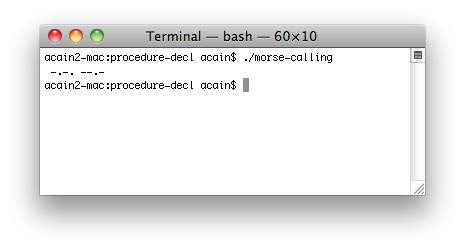
\includegraphics[width=0.9\textwidth]{./topics/procedure-decl/images/MorseCalling} 
   \caption{Morse Calling run in the Terminal}
   \label{fig:procedure-decl-morse_calling}
\end{figure}


\clearpage
\subsection{Program (with Procedures)} % (fold)
\label{sub:program_with_procedures_}

Each Program is a list of instructions (\nameref{sub:statement}s) that command the computer to perform actions. Unfortunately the computer is only able to perform simple actions, meaning that even small programs need many instructions in order to perform their tasks. To help manage these instructions you can group the program's Statements into Procedures, creating Procedures that perform the tasks you need completed in your Program.

\begin{figure}[h]
   \centering
   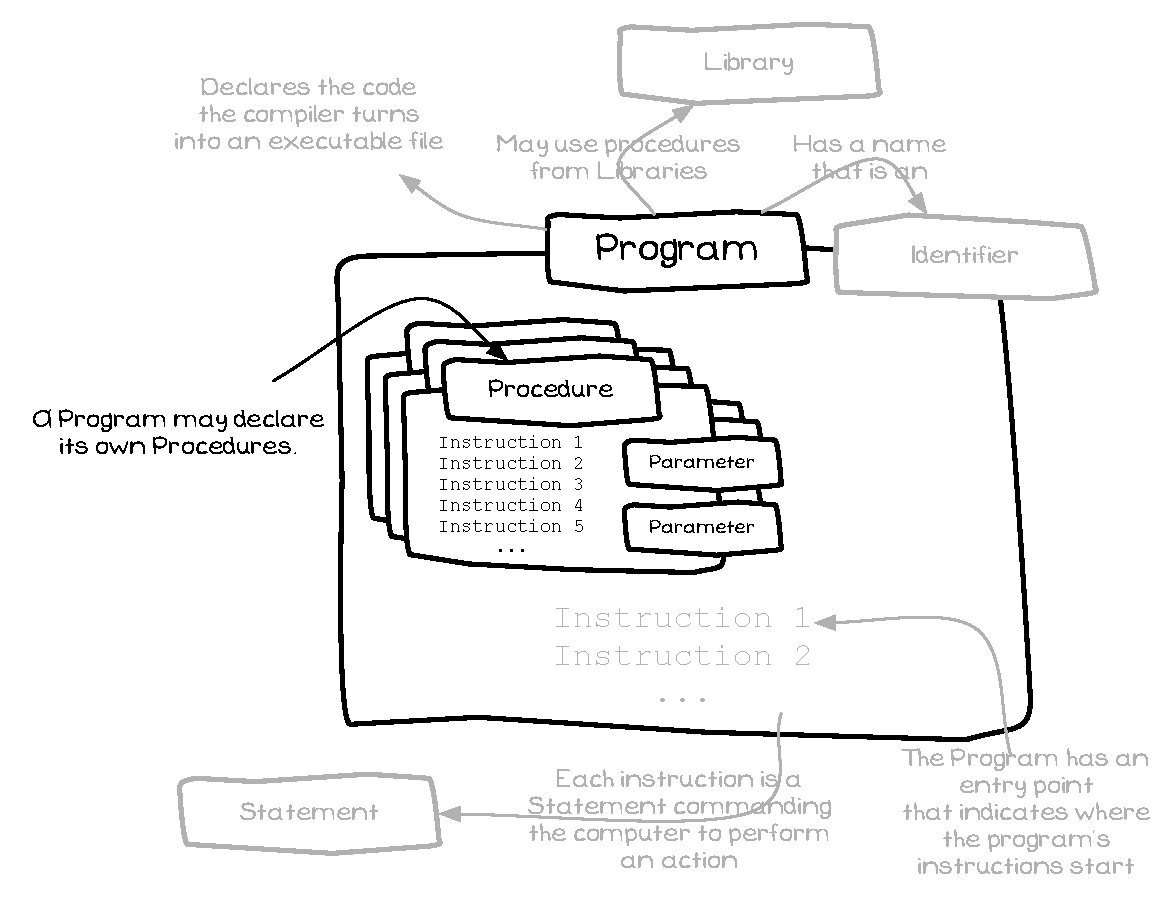
\includegraphics[width=\textwidth]{./topics/procedure-decl/diagrams/ProgramWithProc} 
   \caption{Program with Procedures}
   \label{fig:procedure-decl-program}
\end{figure}

\mynote{
\begin{itemize}
  \item A Program is an \textbf{artefact} that you can \emph{create} in your code.
  \item A Program can contain a number of \nameref{sub:procedure}s.
  \item \nameref{sub:proc_decl-procedure_declarations} allow you to create your own Procedures.
  \item The program's instructions can call the Procedures you create in the program's code.
  \item In C and Pascal the \nameref{sub:proc_decl-procedure_declarations} must appear before they are used in your code.
\end{itemize}
}

% subsection program_with_procedures_ (end)
\clearpage
\subsection{Procedure Declarations} % (fold)
\label{sub:proc_decl-procedure_declarations}

Procedures contain code that define the steps the computer performs when the procedure is called. In your Program you can define your own Procedures, allowing you to divide a Program's tasks into separate Procedures.

\begin{figure}[h]
   \centering
   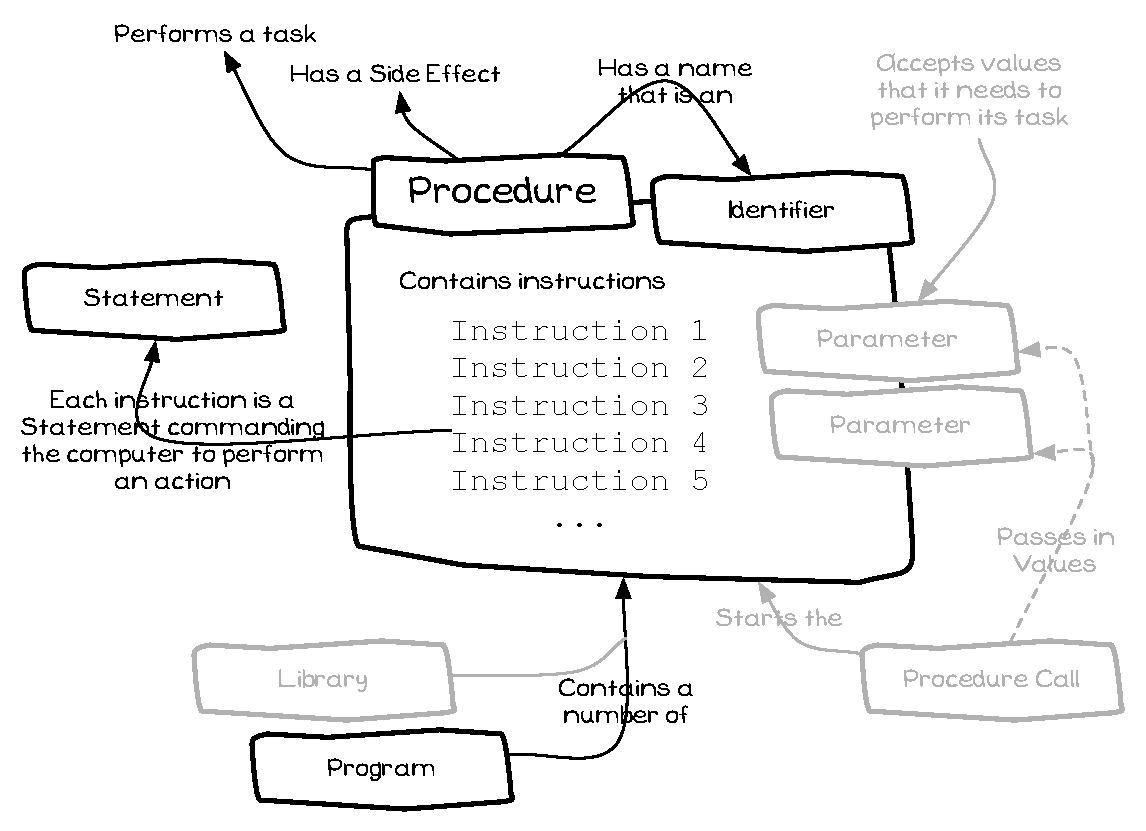
\includegraphics[width=\textwidth]{./topics/procedure-decl/diagrams/ProcedureDeclaration} 
   \caption{Procedure Declaration}
   \label{fig:procedure-decl-procedure-decl}
\end{figure}

\mynote{
\begin{itemize}
  \item A Procedure is an \textbf{artefact} that you can \emph{create} and \emph{use} in your code.
  \item Each Procedure contains code to perform a certain task. When you want the task performed you call the Procedure.
  \item Procedures should have a \textbf{side effect}\footnote{Output to the Terminal is an example of a Side Effect. After calling these procedures the text you wanted to appear was written to the Terminal. These Procedures changed the Terminal.}, meaning that it changes something when it is executed.
  \item The Procedure's declaration defines its \textbf{name}, and the \textbf{steps} it performs.
  \item Each instructions in the Procedure is a \nameref{sec:program-creation-statement}.
  \item The Procedure's \nameref{sec:program-creation-identifier}:
  \begin{itemize}
    \item Is the name used to call the Procedure.
    \item Should be a \textbf{verb} that \textbf{reflects the task} the Procedure performs.
  \end{itemize} 
  \item When the Procedure is called its instructions are executed.
  \item Each Procedure's instructions are isolated from the other code in your Program. When you are working on a Procedure you do not need to know about the internal workings of the other procedures.
\end{itemize}
}

% subsection procedure_declarations (end)

\clearpage
\subsection{Summary} % (fold)
\label{sub:procedure-decl_summary}

This section has introduced you to the idea of creating and using your own Procedures. The concepts related to this are shown in Figure \ref{fig:procedure-decl-summary}. The next section will examine how these concepts can be used to design the Morse Code program.

\begin{figure}[h]
   \centering
   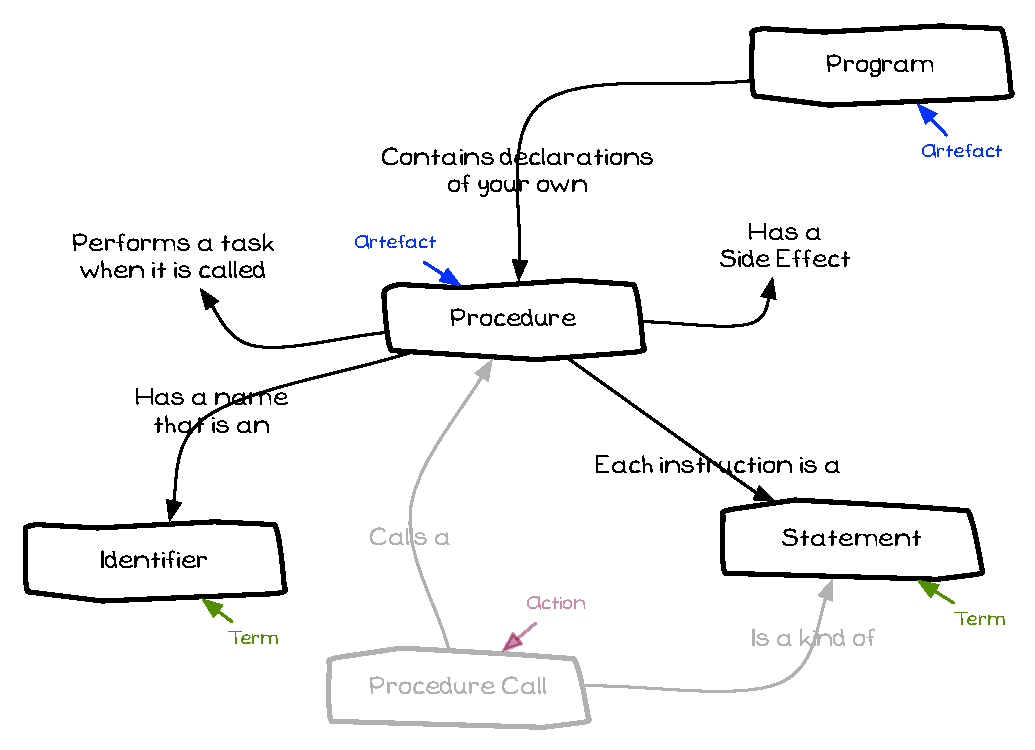
\includegraphics[width=\textwidth]{./topics/procedure-decl/diagrams/Summary} 
   \caption[Chapter Concepts]{Key Concepts introduced in this Chapter}
   \label{fig:procedure-decl-summary}
\end{figure}

\mynote{
\begin{itemize}
  \item \textbf{Artefacts} are things you can \emph{create} and \emph{use}.
  \item \textbf{Terms} are things you need to \emph{understand}.
  \item \textbf{Actions} are things you can \emph{command} the computer to perform.
\end{itemize}
}


% subsection summary (end)


% section procedure_declaration_concepts (end)


% ========================
% = Using these concepts =
% ========================

\clearpage
\section{Using these Concepts} % (fold)
\label{sec:using_these_concepts_procedure_decl}

Procedures give us a means of modelling the tasks we want the computer to perform. Rather than just having a long list of instructions, we can create procedures that contain the steps needed to perform individual tasks that the program must carry out. The program's instructions can then be very simple, just calling the procedures that we have written to carry out the tasks as needed.

\subsection{Designing Morse Calling} % (fold)
\label{sub:designing_morse_calling}

Table \ref{tbl:procedure-decl-morse_calling} contains a description of the next program we are going to design. This program will output a message in Morse Code to the Terminal. In designing this program we will make use of the concepts introduced in this chapter; we will divide the program's code into a number of procedures each with the instructions to get the computer to perform a single task.

\begin{table}[h]
\centering
\begin{tabular}{l|p{10cm}}
  \hline
  \multicolumn{2}{c}{\textbf{Program Description}} \\
  \hline
  \textbf{Name} & \emph{Morse Calling} \\
  \\
  \textbf{Description} & Displays the morse code for `\emph{Calling Anyone}' on the Terminal. \\
  \hline
\end{tabular}
\caption{Description of the Morse Calling program.}
\label{tbl:procedure-decl-morse_calling}
\end{table}

To design and implement this program we need to follow a number of steps:
\begin{enumerate}
  \item Understand the problem, and get some ideas on the tasks that need to be performed.
  \item Choose the artefacts we will create and use
  \item Map these artefacts to code
  \item Compile and run the program
\end{enumerate}

Our first step will be to analyse the problem, and find related material that we can use to make sure we know what the computer needs to do. You need to understand what the program needs to do before you can design the solution. For this program you need to find out a little more about Morse Code so that you can issue the right signals. An important part of this analysis will be to identify the tasks that need to performed in order to meet the programs requirements.

Having understood the problem, the next step will be to create a design for the solution. This involves choosing the artefacts (procedures at this point) that you will \textbf{use}, and the artefacts that you will \textbf{create}. You use the information you gained from analysing the requirements to help you model the tasks that need to be performed in the code.

This is the point where you need to map the artefacts that you need to create to code. You can use the Language Syntax rules to determine what needs to be typed in order to make sure your program will compile.

Finally you can test your program by running it and observing the output. If there are compiler errors then you need to fix these, so that the program compiles. Then you need to check that the output of the program matches the expected outcome. Your understanding of how the program should work will be important during the testing as much as it was during the design and implementation.

\clearpage
\subsection{Understanding Morse Calling} % (fold)
\label{ssub:understanding_morse_calling}

Understanding the problem is the first step toward creating a solution. In this case you need to understand Morse Code so that you can work out what needs to be written to the Terminal. Wikipedia describes Morse Code as a sequence of long and short signals used to encode textual data. When we write this out to the Terminal the short signals can be represented using a dot (.), the long signals using a dash (-). Table \ref{tbl:procedure-decl-morse-codes} contains the Morse code signals for letters, numbers, and some punctuation.

\begin{table}[htbp]
  \centering
  \begin{tabular}{|p{1cm}l|p{1cm}l|p{1cm}l|p{1cm}l|}
    \hline
    \centering A & {\huge \morse a}  & \centering K & {\huge \morse K} & \centering U & {\huge \morse U} & \centering 4 & {\huge \morse 4}\\
    \centering B & {\huge \morse b}  & \centering L & {\huge \morse L} & \centering V & {\huge \morse V} & \centering 5 & {\huge \morse 5}\\
    \centering C & {\huge \morse c}  & \centering M & {\huge \morse M} & \centering W & {\huge \morse W} & \centering 6 & {\huge \morse 6}\\
    \centering D & {\huge \morse d}  & \centering N & {\huge \morse N} & \centering X & {\huge \morse X} & \centering 7 & {\huge \morse 7}\\
    \centering E & {\huge \morse e}  & \centering O & {\huge \morse O} & \centering Y & {\huge \morse Y} & \centering 8 & {\huge \morse 8}\\
    \centering F & {\huge \morse f}  & \centering P & {\huge \morse P} & \centering Z & {\huge \morse Z} & \centering 9 & {\huge \morse 9}\\
    \centering G & {\huge \morse g}  & \centering Q & {\huge \morse Q} & \centering 0 & {\huge \morse 0} & \centering . & {\huge \morse .}\\
    \centering H & {\huge \morse h}  & \centering R & {\huge \morse R} & \centering 1 & {\huge \morse 1} & \centering , & {\huge \morse ,}\\
    \centering I & {\huge \morse i}  & \centering S & {\huge \morse S} & \centering 2 & {\huge \morse 2} & \centering ? & {\huge \morse ?}\\
    \centering J & {\huge \morse j}  & \centering T & {\huge \morse T} & \centering 3 & {\huge \morse 3} & \centering ! & {\huge \morse !}\\
    \hline
  \end{tabular}
  \caption{Morse code signals for letters and numbers}
  \label{tbl:procedure-decl-morse-codes}
\end{table}

With some additional searching you can also find that the signal for `\emph{Calling Anyone}' is the code to signal C and Q. This means that the Program needs to output the signals {\morse CQ} (the signals for C and Q), see Table \ref{tbl:procedure-decl-morse-codes}.

\bigskip

As you read through this information its important to try and identify the tasks that the program will need to perform. These tasks can then be modelled in the program's code. The following list outlines the tasks that can be identified in the above descriptions. Read back over the text and make sure you can see where each of these can be identified.

\begin{itemize}
  \item Perform a Short Signal (a dot)
  \item Perform a Long Signal (a dash)
  \item Signal the Character C
  \item Signal the Character Q
\end{itemize}

When you design the solution for this program you will be able to use this information to determine what needs to be created, and the tasks that each of these performs.

\begin{itemize}
  \item Perform Short Signal will output a dot (.) to the Terminal.
  \item Perform Long Signal will output a dash (-) to the Terminal.
  \item Signal C will perform a Long Signal, then a Short Signal, then a second Long Signal, and a second Short Signal. This will end by printing a space to separate it from the next character.
  \item Signal Q will perform a Long Signal, a second Long Signal, a Short Signal, and then a third Long Signal. This will end by printing a space to separate it from the next character.
\end{itemize}

% subsubsection understanding_morse_calling (end)
\clearpage
\subsection{Choosing Artefacts for Morse Calling} % (fold)
\label{sub:procedure-decl-choosing_artefacts}

Having finished the analysis of the problem, the next step is to design the solution. This will involve determining which programming artefacts you will need to build, and the which programming artefacts exist for you to use. 

\begin{itemize}
  \item Create a \textbf{program} the user can execute. This will signal C and Q using Morse Code. Within this program there are several sub-tasks that can be coded into their own procedures.
  \begin{itemize}
    \item \textbf{Short Signal} - Morse Code needed the ability to perform a short signal. The instructions for this can be coded into a \emph{Short Signal} procedure. In this case that will output a dot (.) to the Terminal.
    \item \textbf{Long Signal} - Similar to the \emph{Short Signal}, this procedure will contain the instructions needed to perform a \emph{Long Signal}, in this case this will output a dash (-) to the Terminal.
    \item \textbf{Signal C} - This task will contain the instructions needed to get the computer to signal the character C. Internally this can call the \emph{Short Signal} and \emph{Long Signal} procedures.
    \item \textbf{Signal Q} - Similar to the \emph{Signal C}, this procedure will contain the instructions needed to signal the character Q. Internally it will use the \emph{Short Signal} and \emph{Long Signal} procedures.
  \end{itemize}
  \item The following procedures already exist and can be used to help implement the procedures mentioned above:
  \begin{itemize}
    \item The language provides a procedure to write data to the Terminal.
  \end{itemize}
\end{itemize}

\csection{In C the procedure to write data to the Terminal is the \texttt{printf} procedure from \texttt{stdio.h}.}
\passection{In Pascal there are two procedures to write data to the Terminal, \texttt{Write} and \texttt{WriteLn}.}

The pseudocode for the \emph{Morse Calling} program is shown in Listing \ref{lst:procedure-decl-MorseCalling-pseudo}, with pseudocode for the \emph{Signal C} procedure in Listing \ref{lst:procedure-decl-signalc-pseudo}, \emph{Signal Q} in Listing \ref{lst:procedure-decl-signalq-pseudo}, and Listing \ref{lst:procedure-decl-shortsignal-pseudo} showing the pseudocode for the \emph{Short Signal} procedure.

\clearpage
\pseudocode{lst:procedure-decl-MorseCalling-pseudo}{Pseudocode for Morse Calling program.}{./topics/procedure-decl/application/MorseCalling.txt}

\pseudocode{lst:procedure-decl-signalc-pseudo}{Pseudocode for the Signal C procedure.}{./topics/procedure-decl/application/SignalC.txt}

\pseudocode{lst:procedure-decl-signalq-pseudo}{Pseudocode for the Signal Q procedure.}{./topics/procedure-decl/application/SignalQ.txt}

\pseudocode{lst:procedure-decl-shortsignal-pseudo}{Pseudocode for the Short Signal procedure.}{./topics/procedure-decl/application/ShortSignal.txt}

\pseudocode{lst:procedure-decl-longsignal-pseudo}{Pseudocode for the Long Signal procedure.}{./topics/procedure-decl/application/LongSignal.txt}

\mynote{
Have a look over the Procedures and the Morse Calling Program and note the following things:
\begin{itemize}
  \item The Procedures appear within the Program.
  \item The name of the procedure indicates what it does.
  \item \texttt{Short Signal} is called by the \texttt{Signal C} and \texttt{Signal Q} procedures.
  \item \texttt{Short Signal} is not directly called by the Program.
  \item The \texttt{SignalC} Procedure calls the \texttt{Long Signal} and \texttt{Short Signal} procedures.
  \item In the C or Pascal code, the Procedure's declaration must appear before its use, so \texttt{Short Signal} and \texttt{Long Signal} will need to appear at the top of the code, \texttt{Signal C} and \texttt{Signal Q} in the middle, and the Program's instructions at the end.
\end{itemize}
}

% subsection choosing_artefacts (end)

\clearpage
\subsection{Writing the Code for Morse Calling} % (fold)
\label{sub:writing_the_code_for_morse_calling}

The pseudocode from section \ref{sub:procedure-decl-choosing_artefacts} \nameref{sub:procedure-decl-choosing_artefacts} shows the instructions, and how these should be divided between a number of custom created procedures. At this stage these instructions need to be translated into source code, so that they can be compiled and the resulting program tested.

The following two sections, Section \ref{sec:procedure_declaration_in_c} \nameref{sec:procedure_declaration_in_c} and Section \ref{sec:procedure_declaration_in_pascal} \nameref{sec:procedure_declaration_in_pascal}, contain a description of the syntax needed to create programs in the C and Pascal programming languages that include Procedure declarations.

Each of these sections will contain extended Program declaration rules that show you where the Procedure Declarations can be coded, along with the rules for how Procedure Declarations should appear.

\mynote{

Remember the basic process for reading the Syntax Diagrams is to:
\begin{enumerate}
  \item Find the page with the Syntax rule you are interested in knowing about.
  \item Have a quick look at the Syntax Diagram and the rules it contains. Read each rule, and get a basic feel for how it is going to come together for your program.
  \item Read the example to see one way of using the Rule. The Syntax Diagram can be used to create any number of variations of the rule, the example gives you at least one way these rules can be coded.
  \item Return to the diagram and make sure you can match each part of the example back to the rule that created it.
  \item Now look up any related rules that are not explained on this rule's page. For example, a \nameref{sub:program_with_procedures_} uses the \nameref{sub:proc_decl-procedure_declarations} rule, you will need to read this rule to determine how to declare the Procedures you want to create in the code.
\end{enumerate}

}

% subsection writing_the_code_for_morse_calling (end)
\subsection{Compiling and Running Morse Calling} % (fold)
\label{sub:compiling_and_running_morse_calling}

Once you have completed your program, you need to compile and test it. 

\begin{enumerate}
  \item Open the \textbf{Terminal}\footnote{The \textbf{MinGW Shell} on Windows.} program for your Operating System
  \item Use the \texttt{\textbf{cd}} command to move to the directory with your code, for example \newline \bashsnipet{cd /Users/acain/Documents/Code}
  \item Run the compiler with your program's code. See the language specific details below.
  \item Fix any compiler errors, using the tips from Section \ref{ssub:compiler_errors} \nameref{ssub:compiler_errors}.
  \item Execute the program using \bashsnipet{./MorseCalling} and check the results
\end{enumerate}

\csection{
The C compiler is called \textbf{gcc}. To compile your \emph{Morse Calling} program you will need to run the following: \newline \newline \bashsnipet{gcc -o MorseCalling morse-calling.c}
}

\passection{
The Pascal compiler is called \textbf{fpc}. To compile your \emph{Morse Calling} program you will need to run the following: \newline \newline \bashsnipet{fpc -S2 MorseCalling.pas}
}



% subsection compiling_and_running_morse_calling (end)


% subsection designing_morse_calling (end)


% section using_these_concepts (end)

% =============
% = C Section =
% =============

\cleardoublepage
\def\pageLang{c}
\section{Procedure Declarations in C} % (fold)
\label{sec:procedure_declaration_in_c}

% Concept overview
\subsection{Implementing Morse Calling in C} % (fold)
\label{sub:implementing_morse_calling_in_c}

Section \ref{sec:using_these_concepts_procedure_decl} of this chapter introduced the `Morse Calling' program, and its design. Its implementation requires the definition of some procedures in the Program's code. This section of the chapter introduces the C syntax rules for declaring your own procedures, with the C implementation of Morse Calling being shown in Listing \ref{lst:procedure-decl-c-morse_calling}.

\csection{\ccode{lst:procedure-decl-c-morse_calling}{C Morse Calling}{code/c/procedure-decl/morse-calling.c}}

\mynote{
\begin{itemize}
  \item Save the C code in a file named \texttt{morse-calling.c}.
  \item Compile this using \bashsnipet{gcc -o MorseCalling morse-calling.c}.
  \item Run the resulting program using \bashsnipet{./MorseCalling}.
  \item Check that the output matches the expected values.
  \item Looking over the code you should be able to see the instructions for each Procedure.
  \item Notice how the indentation makes it easy to see where each Procedure starts and ends. Always lay your code out so that it is easy to see its structure.
  \item See how the procedures are declared before they are used. This is important as the C compiler must know about the Procedure before you can call it.
  \item To see how to create this have a look at the Syntax for declaring \nameref{sub:c_program_with_procedures_}.
  \item The Program's declaration can contain a number of Procedures using the \nameref{sub:c_procedure_declaration} syntax.
\end{itemize}
}

% subsection implementing_morse_sos_in_c (end)

% Parts of the syntax
\clearpage
\subsection{C Program (with Procedures)} % (fold)
\label{sub:c_program_with_procedures_}

The C code for a Program contains the program's instructions in \texttt{main}, along with your procedure declarations.

\csyntax{csynt:procedure-decl-program}{a Program (with procedures)}{procedure-decl/program-with-procedures}

\csection{\ccode{lst:program-c-say-hello-proc}{Is Anyone There?}{code/c/procedure-decl/say-hello-proc.c}}

\mynote{
\begin{itemize}
  \item The header includes, main function, and block are all the same as previously seen.
  \begin{itemize}
    \item The \emph{header include} gives you access to the Standard IO library.
    \item The \emph{main function} is the entry point for your program, it contains the instructions that are followed when the program is launched.
    \item The \emph{block} contains the instructions used within the \texttt{main} function.
  \end{itemize}
  \item You can place \textbf{declarations} after the \emph{header includes} and before the \emph{main function}.
  \item The \emph{declarations} can contain any number of \emph{procedure declarations}. See \nameref{sub:c_procedure_declaration} for details on this code.
  \bigskip
  \item The code in Listing \ref{lst:program-c-say-hello-proc} shows a Program with two procedures: \texttt{say\_hello()} and \texttt{say\_is\_anyone\_there()}.
  \item Notice that these procedures are declared after the \emph{header include} \csnipet{#include <stdio.h>} and before the \emph{main function}.
\end{itemize}
}



% subsection c_program_with_procedures_ (end)
\clearpage
\subsection{C Procedure Declaration} % (fold)
\label{sub:c_procedure_declaration}

The Syntax for a C Procedure Declaration is shown in Figure \ref{csynt:procedure-decl-procedure-decl}.

\csyntax{csynt:procedure-decl-procedure-decl}{a Procedure}{procedure-decl/procedure-decl}

\csection{\ccode{lst:program-c-print-steps}{Cooking a Meal}{code/c/procedure-decl/print-steps.c}}

\mynote{
\begin{itemize}
  \item There are three Procedures declared in the code in Listing \ref{lst:program-c-print-steps}.
  \item A \textbf{Procedure Declaration} starts with the word \textbf{\texttt{void}}. This indicates that the following code is a procedure declaration to the compiler.
  \item The \textbf{Procedure Name} is an identifier. It is the name of the Procedure. This can be any valid \nameref{sub:c_identifier} that has not been used before.
  \item The empty parenthesis must appear after the procedure's name, and before the \emph{block}.
  \item The \textbf{block} should look familiar. This is the same as was used in the \emph{main function} of the program to define its instructions, and is used for the same purpose within the \emph{Procedure Declaration}.
  \bigskip
  \item There are a number of conventions, called coding standards, that describe how your code should appear for a given language. In this text we will use a common C convention of having all \emph{Procedure Names} in \textbf{lower case}, with underscores ( \_ ) used to separate words. So the \emph{Get Ingredients} procedure becomes \texttt{get\_ingregients}.
\end{itemize}
}

% subsection c_procedure_declaration (end)


% section procedure_declaration_in_c (end)


% ==================
% = Pascal Section =
% ==================

\cleardoublepage
\def\pageLang{pas}
\section{Procedure Declarations in Pascal} % (fold)
\label{sec:procedure_declaration_in_pascal}

% Concept overview
\subsection{Implementing Morse Calling in Pascal} % (fold)
\label{sub:implementing_morse_calling_in_pascal}

Section \ref{sec:using_these_concepts_procedure_decl} of this chapter introduced the `Morse Calling' program, and its design. Its implementation requires the definition of some procedures in the program's code. This section of the chapter introduces the Pascal syntax rules for declaring your own procedures, with the Pascal implementation of Morse Calling being shown in Listing \ref{lst:procedure-decl-pas-morse_calling}.

\passection{\pascode{lst:procedure-decl-pas-morse_calling}{Pascal Morse Calling}{code/pascal/procedure-decl/MorseCalling.pas}}

\mynote{
\begin{itemize}
  \item Save the Pascal code in a file named \texttt{MorseCalling.pas}.
  \item Compile this using \bashsnipet{fpc -S2 MorseCalling.pas}.
  \item Run the resulting program using \bashsnipet{./MorseCalling}.
  \item Check that the output matches the expected values.
  \item Looking over the code you should be able to see the instructions for each procedure.
  \item Notice how the indentation makes it easy to see where each procedure starts and ends. Always lay your code out so that it is easy to see its structure.
  \item See how the procedures are declared before they are used. This is important as the Pascal compiler must know about procedures before you can call them.
  \item To see how to create this have a look at the syntax for declaring \nameref{sub:pas_program_with_procedures_}.
  \item The program's declaration can contain a number of procedures using the \nameref{sub:pas_procedure_declaration} syntax.
\end{itemize}
}

% subsection implementing_morse_sos_in_c (end)

% Parts of the syntax
\clearpage
\subsection{Pascal Program (with Procedures)} % (fold)
\label{sub:pas_program_with_procedures_}

The Pascal code for a program contains the program's instructions, along with your own procedure declarations.

\passyntax{passynt:procedure-decl-program}{a program (with procedures)}{procedure-decl/program-with-procedures}

\passection{\pascode{lst:program-pas-say-hello-proc}{Is Anyone There?}{code/pascal/procedure-decl/SayHelloProc.pas}}

\mynote{
\begin{itemize}
  \item Within your program you can declare your own procedures. 
  \item See \nameref{sub:pas_procedure_declaration} for the syntax to declare your own procedures.
  \item Listing \ref{lst:program-pas-say-hello-proc} shows a program with three procedures: \texttt{Main}, \texttt{ SayHello()}, and \texttt{ SayIsAnyoneThere()}.
  \item Procedures are declared between the \emph{program's header} and the \emph{program's statements}.
\end{itemize}
}



% subsection c_program_with_procedures_ (end)
\clearpage
\subsection{Pascal Procedure Declaration} % (fold)
\label{sub:pas_procedure_declaration}

The syntax for a Pascal procedure declaration is shown in \fref{passynt:procedure-decl-procedure-decl}.

\passyntax{passynt:procedure-decl-procedure-decl}{a procedure}{procedure-decl/procedure-decl}

\passection{\pascode{lst:program-pas-print-steps}{Cooking a meal}{code/pascal/procedure-decl/PrintSteps.pas}}

\mynote{
\begin{itemize}
  \item There are four procedures declared in the code in \lref{lst:program-pas-print-steps}.
  \item A \textbf{procedure declaration} starts with the word \textbf{\texttt{procedure}}. This indicates to the compiler that the following code is a procedure declaration.
  \item The \textbf{procedure's name} is an identifier. This can be any valid \nameref{sub:pas_identifier} that has not been used before.
  \item The empty parenthesis must appear after the procedure's name, and before the semicolon and the \emph{block}.
  \bigskip
  \item There are a number of conventions, called coding standards, that describe how your code should appear for a given language. In this text we will use a common Pascal convention of having all \emph{procedure names} in \textbf{Pascal Case}, this uses an uppercase character for the first letter of each word in the identifier. So the \emph{Get Ingredients} procedure becomes \texttt{GetIngregients}.
\end{itemize}
}

% subsection c_procedure_declaration (end)


% section procedure_declaration_in_c (end)


% =========================
% = Understanding Section =
% =========================
\clearpage
\def\pageLang{none}
\section{Understanding Procedure Declaration and Calls} % (fold)
\label{sec:understanding_procedure_declaration_and_calls}

This Chapter has introduced the idea of creating Procedures within your program's code. These procedures can be used to implement the different tasks that you want your program to perform. 

This Section will help you answer the following questions:
\begin{itemize}
  \item How can I visualise the Procedures within a program?
  \item What happens when my Procedures are called?
\end{itemize}

\subsection{Visualising Procedures in Morse Calling} % (fold)
\label{sub:visualising_morse_calling}

When you are writing the code, the internal details of how a Procedure works are important. But, it is equally important to be able to picture how these procedures interact within the program as a whole. One technique for visualising this is to draw a \textbf{Structure Chart}.

A \emph{Structure Chart} is a diagram that has two elements: rectangles representing the procedures in your code, and arrows representing calls. The Structure Chart for the Morse Calling program is shown in Figure \ref{fig:procedure-decl-morsecalling-structure}. In this you can see that the Morse Calling program has four main procedures that implement its functionality, in addition to the program's main logic: the \texttt{Signal C}, \texttt{Signal Q}, \texttt{Long Signal}, and \texttt{Short Signal} procedures. It also shows that the program's main logic calls \texttt{Signal C} and \texttt{Signal Q}, that \texttt{Signal C} calls \texttt{Long Signal} and \texttt{Short Signal}, as does \texttt{Signal Q}.

\begin{figure}[htbp]
   \centering
   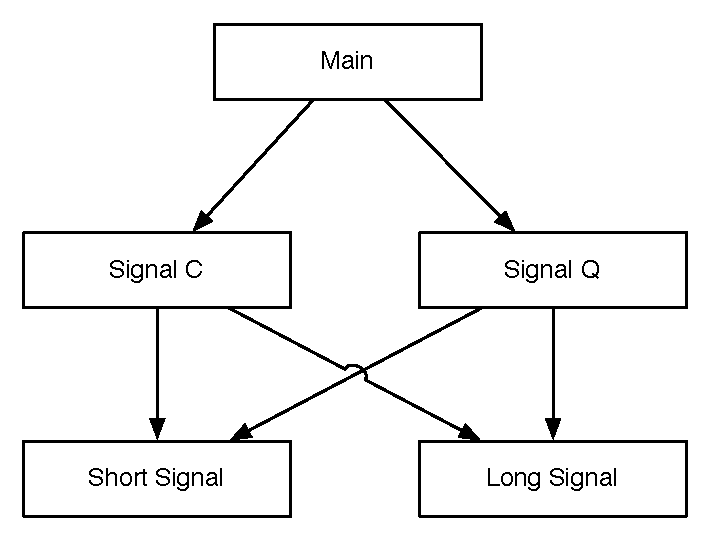
\includegraphics[width=0.75\textwidth]{./topics/program-creation/diagrams/MorseCallingStructureChart} 
   \caption{Structure Chart showing the Procedures in Morse Calling}
   \label{fig:procedure-decl-morsecalling-structure}
\end{figure}

The rectangles in the Structure Chart represent the Procedures. As the name of the procedure should reflect its task/actions this means that the reader of the diagram can get some insight into what the program is doing, and how it is achieving its tasks. From Morse Calling's Structure Chart you can see that the program is Signalling the character's \emph{C} and \emph{Q}, which internally use \emph{Long} and \emph{Short} signals to achieve their tasks.

The arrows in the Structure Chart show procedure calls. The arrow from the \texttt{Signal C} procedure to \texttt{Long Signal} tells us that somewhere in the code for \texttt{Signal C} there is one or more calls to \texttt{Long Signal}. There is no indication of the order, or frequency, of these calls. Its just simply saying that \texttt{Signal C} calls \texttt{Long Signal}.

The Structure Chart is useful for getting an overall picture of how the program is structured. It can help the designer communicate such things as \emph{What Procedures are there in this program?} and \emph{How are these Procedures related to each other?} It helps developers new to the project to get a feeling for how the code is distributed within the solution, and to know where the core logic can be found. It also provides a means of determining the impact of changing the functionality of the tasks in the program. For example, if you change how \texttt{Long Signal} works that may impact on \texttt{Signal C} and on \texttt{Signal Q}. Any changes you made here would mean you needed to test that \texttt{Signal C} and \texttt{Signal Q} still worked as expected.

\bigskip

The Structure Chart is a great communication tool for getting an overall picture of how a solution fits together, but it only shows the \textbf{static structure}. Communicating things about the code, but not things about how the code executed. An effective designer will want to communicate both the \emph{static structure}, as well as the \textbf{dynamic behaviour} of the solution. To communicate these details you need to look for complementary techniques.

% sub:visualising_morse_calling (end)

\subsection{Visualising procedure calls in Morse Calling} % (fold)
\label{sub:visualising_procedure_calls_in_morse_calling}

The Structure Chart communicates the static structure of the solution, showing the Procedures and their relationships but lacking any details on how this structure works dynamically. This dynamic information can be captured in a \textbf{Sequence Diagram}, which works together with the Structure Chart to complete the overview of the program's structure and dynamic behaviour.

Figure \ref{fig:procedure-decl-morsecalling-sequence} shows the \emph{Sequence Diagram} for the Morse Calling program. This shows the \emph{procedure calls} that will occur within an execution of the program's code. The Sequence Diagram shows the order in which procedure calls occur, with time travelling down the page and the calls travelling across. 

\begin{figure}[htbp]
   \centering
   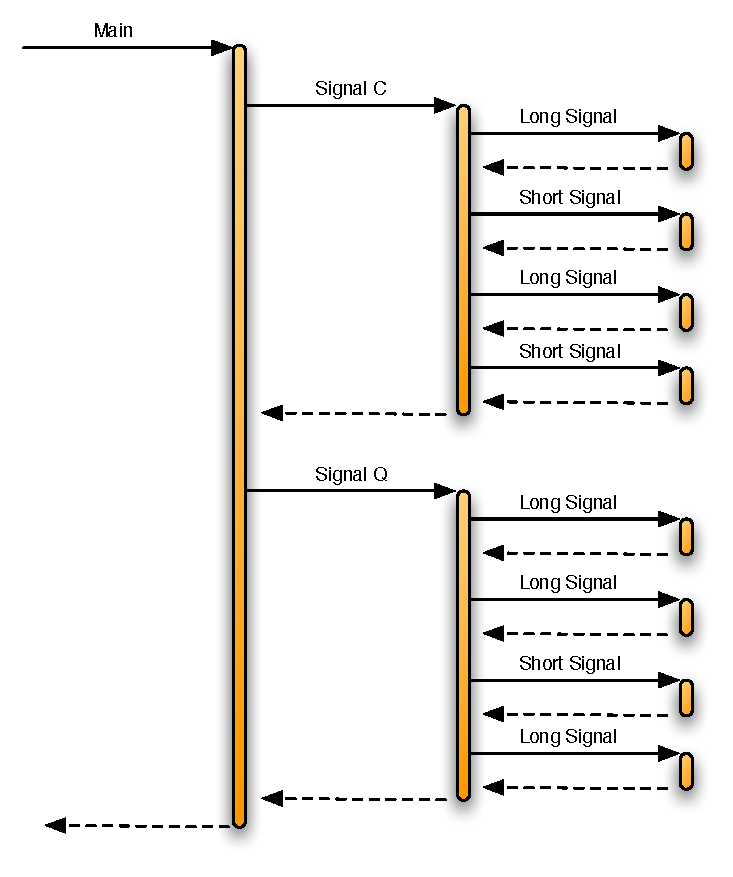
\includegraphics[width=0.75\textwidth]{./topics/program-creation/diagrams/MorseCallingSequenceDiagram} 
   \caption{Sequence Diagram for Morse Calling}
   \label{fig:procedure-decl-morsecalling-sequence}
\end{figure}

You start reading this diagram from the top, with each arrow representing the call to a Procedure, and the thin vertical rectangles representing the time taken for the called procedure to complete its task. Reading the Sequence Diagram for Morse Calling you can see that the first thing to occur is the \texttt{Main} body of the program's code is started. The arrow from the far left indicates that something, in this case being the user launching the program, starts this code running.

The first thin vertical rectangle is the program's main instructions, and its first action is to call \texttt{Signal C} as shown by the arrow pointing to the second vertical bar. This is our first procedure call, the program's instructions call \texttt{Signal C}. Notice that at this point there are two vertical bars. These represent the two frames on the Stack, and show us that when \texttt{Signal C} finishes the execution will return to the program's main instructions.

Within \texttt{Signal C} the first action is to call \texttt{Long Signal}, as shown be the arrow. Time-wise this is the second procedure call. First the Main code called \texttt{Signal C}, which in turn called \texttt{Long Signal}. The details on the diagram show us that \texttt{Long Signal} does not call any other procedures that we created. Notice that we have avoided putting in the call to the output procedure to allow us to focus on the Procedures we have created. At this point there are three frame's on the Stack, the first for the \texttt{Main} code, second for \texttt{Signal C}, and third for \texttt{Long Signal}. You can see these if you turn your head on the side. Notice the notice that the vertical bars will mirror the stack.

As \texttt{Long Signal} does not call any other Procedures that we created there are no calls coming out from this procedure's execution. The actions within this code will be performed, and then \texttt{Long Signal} will end. This is shown by the ending of the vertical bar, and a dashed returning arrow showing where the code returns to. This tells us that when \texttt{Long Signal} ends at this point, the computer returns to execute the next instruction in \texttt{Signal C}.

The next instruction in \texttt{Signal C} is the call to \texttt{Short Signal}. Once again this is shown with the calling arrow, and a vertical bar is added to show the steps of the \texttt{Short Signal} executing. \texttt{Short Signal} does not call any other Procedures we created so it ends without any additional calls occurring, and control returns to \texttt{Signal C}.

This process continues, with the diagram showing that \texttt{Long Signal} is called again followed by a call to \texttt{Short Signal}, and then \texttt{Signal C} ends. At this point control returns to the program's main code, where the next call starts \texttt{Signal Q} running. Within \texttt{Signal Q} you can see two calls to \texttt{Long Signal}, followed by a call to \texttt{Short Signal}, and a final call to \texttt{Long Signal}. When the final call to \texttt{Long Signal} ends this marks the end of the \texttt{Signal Q} procedures, and the end of the program's instructions as a whole.

As you can see from the above text the Sequence Diagram communicates a large amount of detail in a relatively small space. Trying to communicate the calling sequence in words is far harder than doing so in a diagram like this. The Sequence Digram allows software designers to communicate the dynamic behaviour of a software solution.

One issue with a Sequence Diagram is that it can quickly become very large if you use it to try and explain all of the actions within a program. As the complexity of your programs grow you will see that it becomes more and more difficult to try to communicate all of the program's behaviour in a single diagram. Instead of trying to communicate the entire program's behaviour, effective Software Designers will use Sequence Diagrams to communicate important details that may be missed otherwise. Focusing on areas where the interaction between the procedures is particularly important. As you progress as a Software Developer see if you can use these diagrams to effectively communicate important points in your designs.

\bigskip

Together \emph{Structure Charts} and \emph{Sequence Diagrams} allow Software Designers to communicate the static structure and dynamic behaviour of their designs. As a software developer you will need to understand how to read these diagrams, and use them to communicate your designs decisions.

% subsection visualising_procedure_calls_in_morse_calling (end)

\subsection{procedure calls in Action} % (fold)
\label{sub:procedure_calls_in_action}

The Sequence Diagram gives you a way of visualising what happens at run time, but let us return to our virtual computer and see how these actions actually work within the computer. 

\begin{enumerate}
  \item \nameref{ssub:morse_calling_is_loaded_into_memory}
  \item \nameref{ssub:signal_c_is_called}
  \item \nameref{ssub:long_signal_is_called}
  \item \nameref{ssub:control_returns_to_signal_c}
  \item \nameref{ssub:short_signal_is_called}
  \item \nameref{ssub:short_signal_ends}
\end{enumerate}

\clearpage
\subsubsection{Morse Calling is Loaded into Memory} % (fold)
\label{ssub:morse_calling_is_loaded_into_memory}

When the program is launched the Operating System loads the code for Morse Calling into memory, and starts it executing in the program's entry point. 

\begin{figure}[htbp]
   \centering
   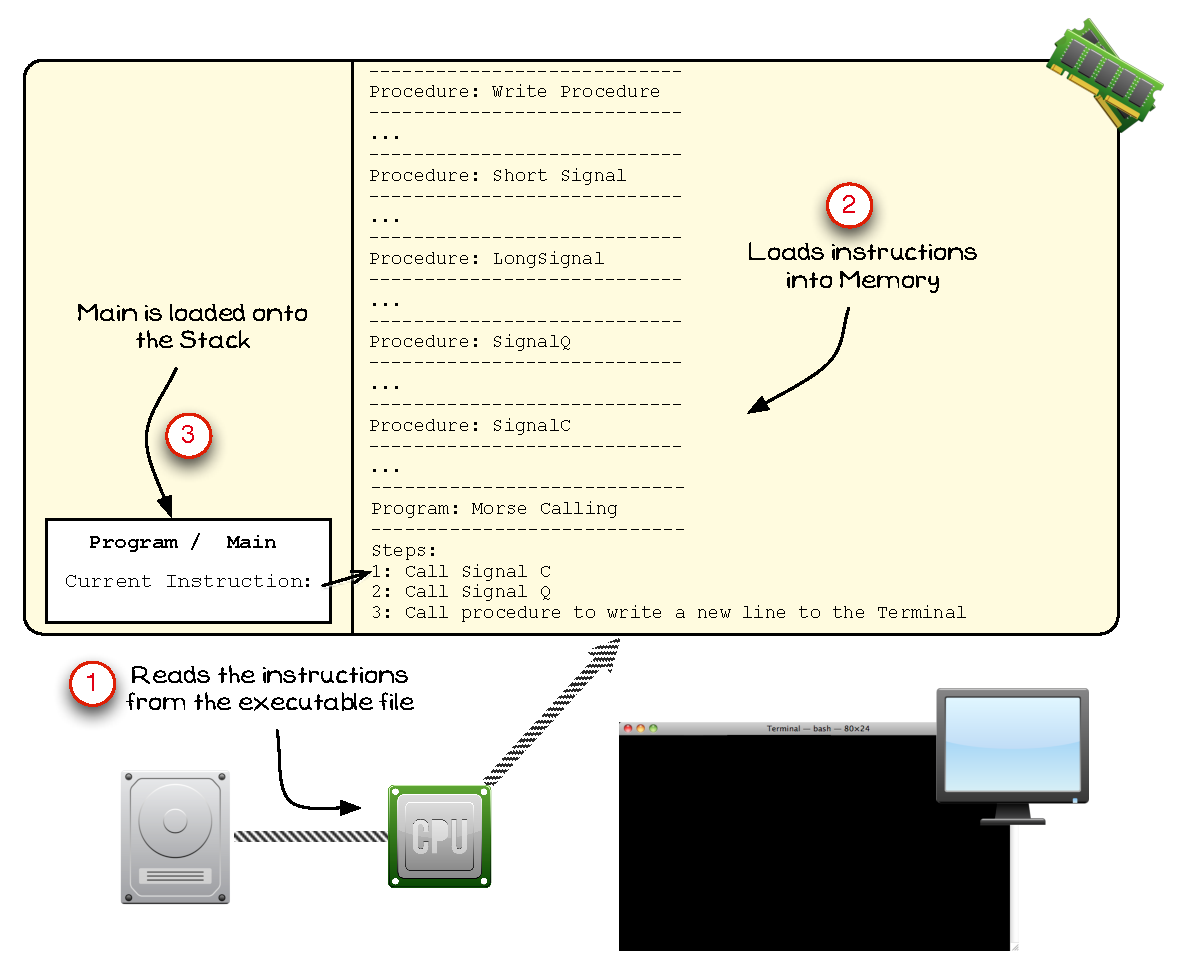
\includegraphics[width=\textwidth]{./topics/program-creation/images/ProcExe1} 
   \caption{The Operating System loads the code for Morse Calling into memory}
   \label{fig:procedure-decl-visualise-morsecalling-1}
\end{figure}

\mynote{
\begin{itemize}
  \item In Figure \ref{fig:procedure-decl-visualise-morsecalling-1} the indicated areas show the following:
  \begin{enumerate}
    \item The Operating System reads the code from the Morse Calling executable.
    \item This code is then loaded into the program's memory.
    \item A frame is added to the Stack for the entry point, the start of the program's instructions.
  \end{enumerate}
  \bigskip
  
  \item The memory for the program is divided into areas for the \textbf{stack}, and the \textbf{code}.
  \item Only part of the program's code is shown in Figure \ref{fig:procedure-decl-visualise-morsecalling-1}, but in reality all of the program's code is loaded into memory.
\end{itemize}
}

% subsubsection morse_calling_is_loaded_into_memory (end)

\clearpage
\subsubsection{Signal C is Called} % (fold)
\label{ssub:signal_c_is_called}

The first action in the program's code is a procedure call that starts the code in \texttt{Signal C} running. 

\begin{figure}[htbp]
   \centering
   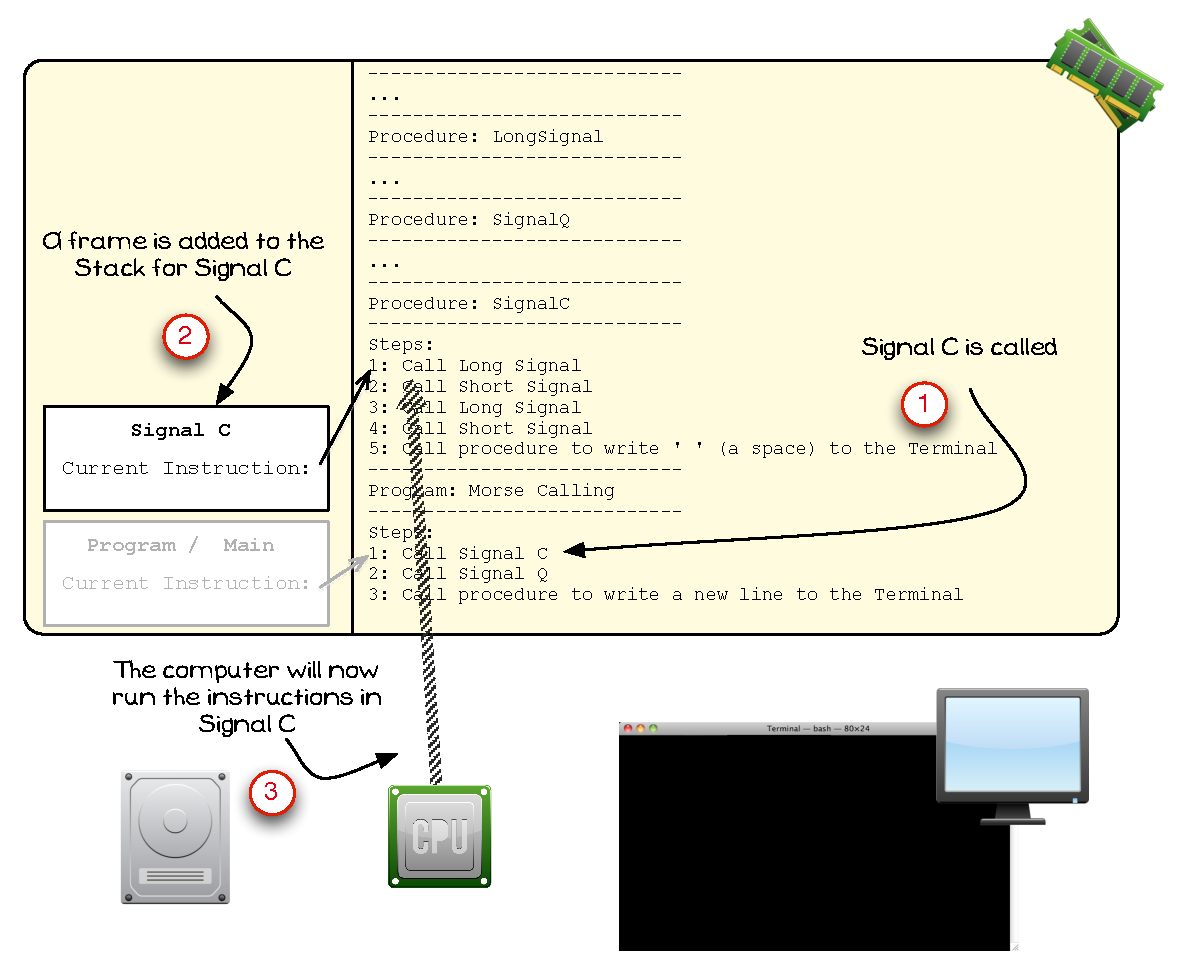
\includegraphics[width=\textwidth]{./topics/program-creation/images/ProcExe2} 
   \caption{The first instruction calls \texttt{Signal C}}
   \label{fig:procedure-decl-visualise-morsecalling-2}
\end{figure}

\mynote{
\begin{itemize}
  \item In Figure \ref{fig:procedure-decl-visualise-morsecalling-2} the indicated areas show the following:
  \begin{enumerate}
    \item The first instruction in the program's is a call to \texttt{Signal C}.
    \item When this is executed a frame is added to the Stack to keep track of the current instruction within \texttt{Signal C}'s code.
    \item As \texttt{Signal C} is now on top of the Stack its instructions are executed. The first instruction in \texttt{Signal C} is a call to \texttt{Long Signal}.
  \end{enumerate}
  \bigskip
  
  \item Notice that the previous Stack Frame keeps track of where the instructions return when \texttt{Signal C} finishes.
  \item The computer runs each instruction one at a time, using the stack to remember where to return when the current Procedure ends.
\end{itemize}
}


% subsubsection signal_c_is_called (end)

\clearpage
\subsubsection{Long Signal is Called} % (fold)
\label{ssub:long_signal_is_called}

The first action in \texttt{Signal C} is to call \texttt{Long Signal}.

\begin{figure}[htbp]
   \centering
   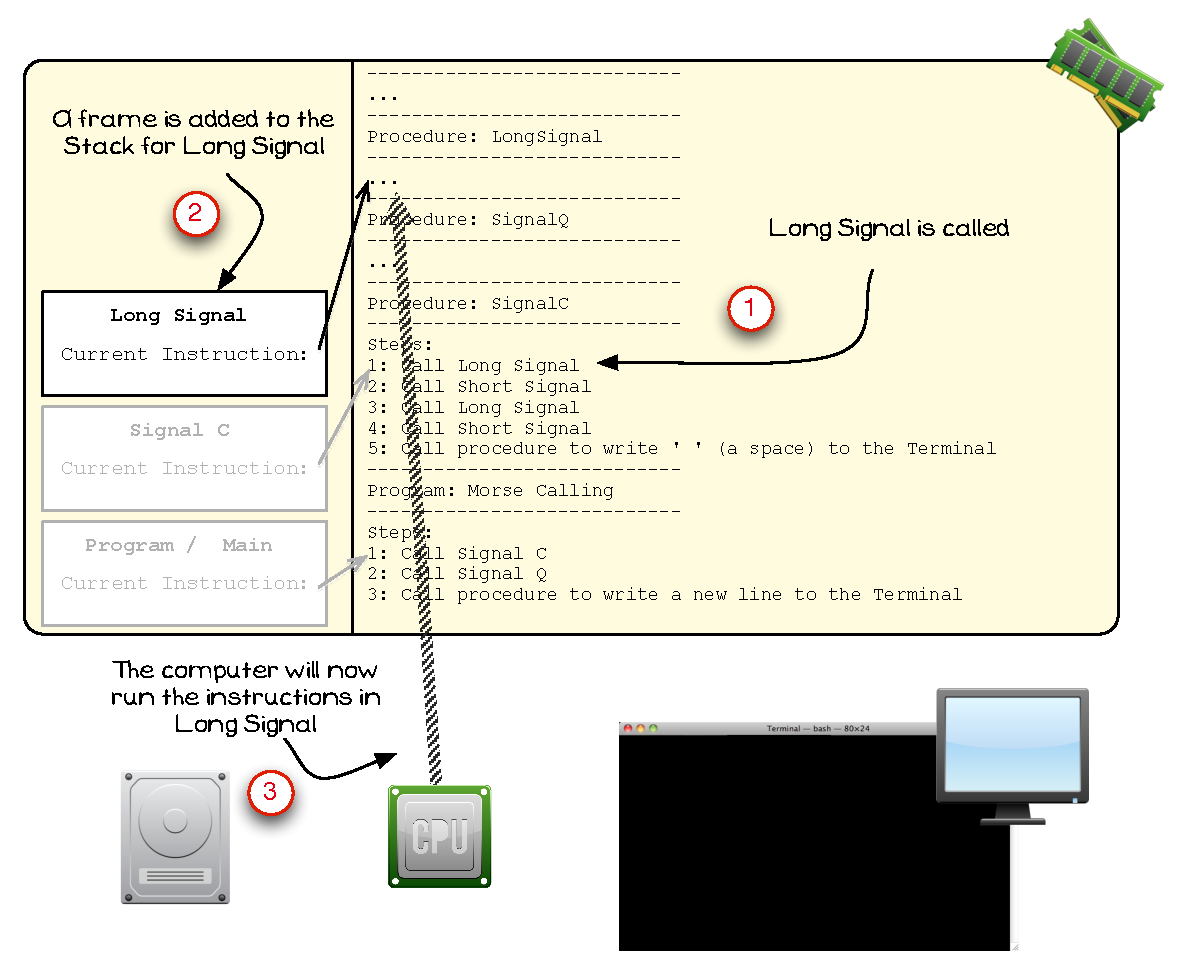
\includegraphics[width=\textwidth]{./topics/program-creation/images/ProcExe3} 
   \caption{Within \texttt{Signal C} the first instruction is to call \texttt{Long Signal}}
   \label{fig:procedure-decl-visualise-morsecalling-3}
\end{figure}

\mynote{
\begin{itemize}
  \item In Figure \ref{fig:procedure-decl-visualise-morsecalling-3} the indicated areas show the following:
  \begin{enumerate}
    \item The first instruction in the \texttt{Signal C} is a call to \texttt{Long Signal}.
    \item When this is executed a frame is added to the Stack to keep track of the current instruction within \texttt{Long Signal}'s code.
    \item As \texttt{Long Signal} is now on top of the Stack its instructions are executed.
  \end{enumerate}
  \bigskip
  
  \item Notice that the previous Stack Frames remain on the Stack to keep track of where the instructions return when \texttt{Long Signal} and \texttt{Signal C} finish.
  \item The computer runs each instruction one at a time, using the stack to remember where to return when the current Procedure ends.
  \item If you look at the Stack you can see that \texttt{Main} called \texttt{Signal C} that called \texttt{Long Signal}. Flip back and have a look at the \nameref{fig:procedure-decl-morsecalling-sequence}, notice that the arrows at the start of the diagram match the current state of the Stack.
\end{itemize}
}

% subsubsection long_signal_is_called (end)

\clearpage
\subsubsection{Control Returns to Signal C} % (fold)
\label{ssub:control_returns_to_signal_c}

When \texttt{Long Signal} finishes running, it has written an underscore to the Terminal, and control returns back to \texttt{Signal C}.

\begin{figure}[htbp]
   \centering
   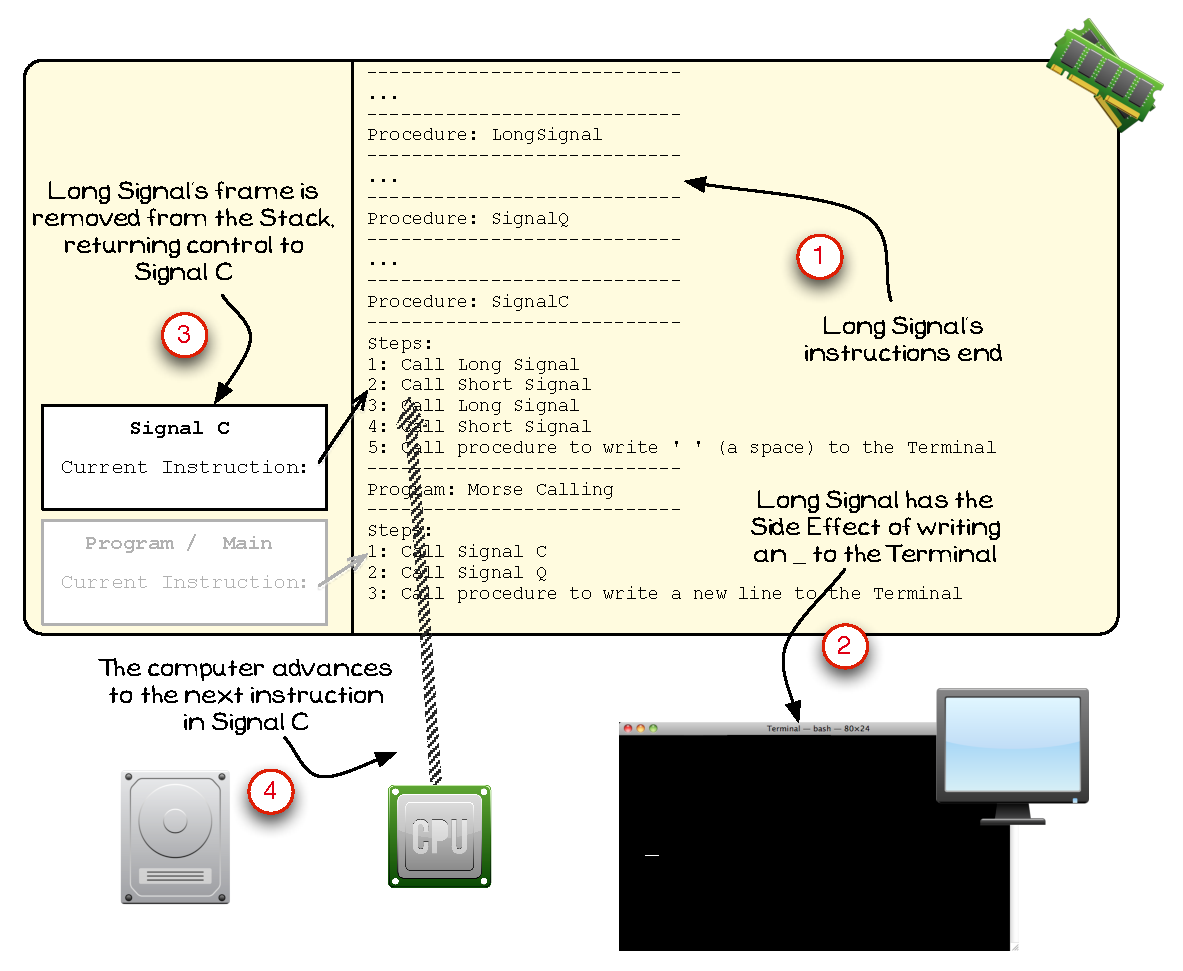
\includegraphics[width=\textwidth]{./topics/program-creation/images/ProcExe4} 
   \caption{\texttt{Long Signal}'s instructions end, returning control to \texttt{Signal C}}
   \label{fig:procedure-decl-visualise-morsecalling-4}
\end{figure}

\mynote{
\begin{itemize}
  \item In Figure \ref{fig:procedure-decl-visualise-morsecalling-4} the indicated areas show the following:
  \begin{enumerate}
    \item The computer runs the instructions in \texttt{Long Signal} until they end.
    \item \texttt{Long Signal} has the \textbf{side effect} of writing an underscore to the Terminal.
    \item When \texttt{Long Signal}'s instructions end control returns to \texttt{Signal C}.
    \item The computer now advanced to the next instruction in \texttt{Signal C}.
  \end{enumerate}
  \bigskip
  
  \item Procedures should have side effects, changing something as a result of being called.
  \item \texttt{Signal C} is now at its second instruction as the computer has finished its first instruction.
  \item In the \nameref{fig:procedure-decl-morsecalling-sequence} the program is now at the point after the first returning\footnote{The dashed arrow returned back from \texttt{Long Signal}.} arrow and is now about to call \texttt{Short Signal}.
\end{itemize}
}


% subsubsection control_returns_to_signal_c (end)

\clearpage
\subsubsection{Short Signal is Called} % (fold)
\label{ssub:short_signal_is_called}

The second action in \texttt{Signal C} is to call \texttt{Short Signal}.

\begin{figure}[htbp]
   \centering
   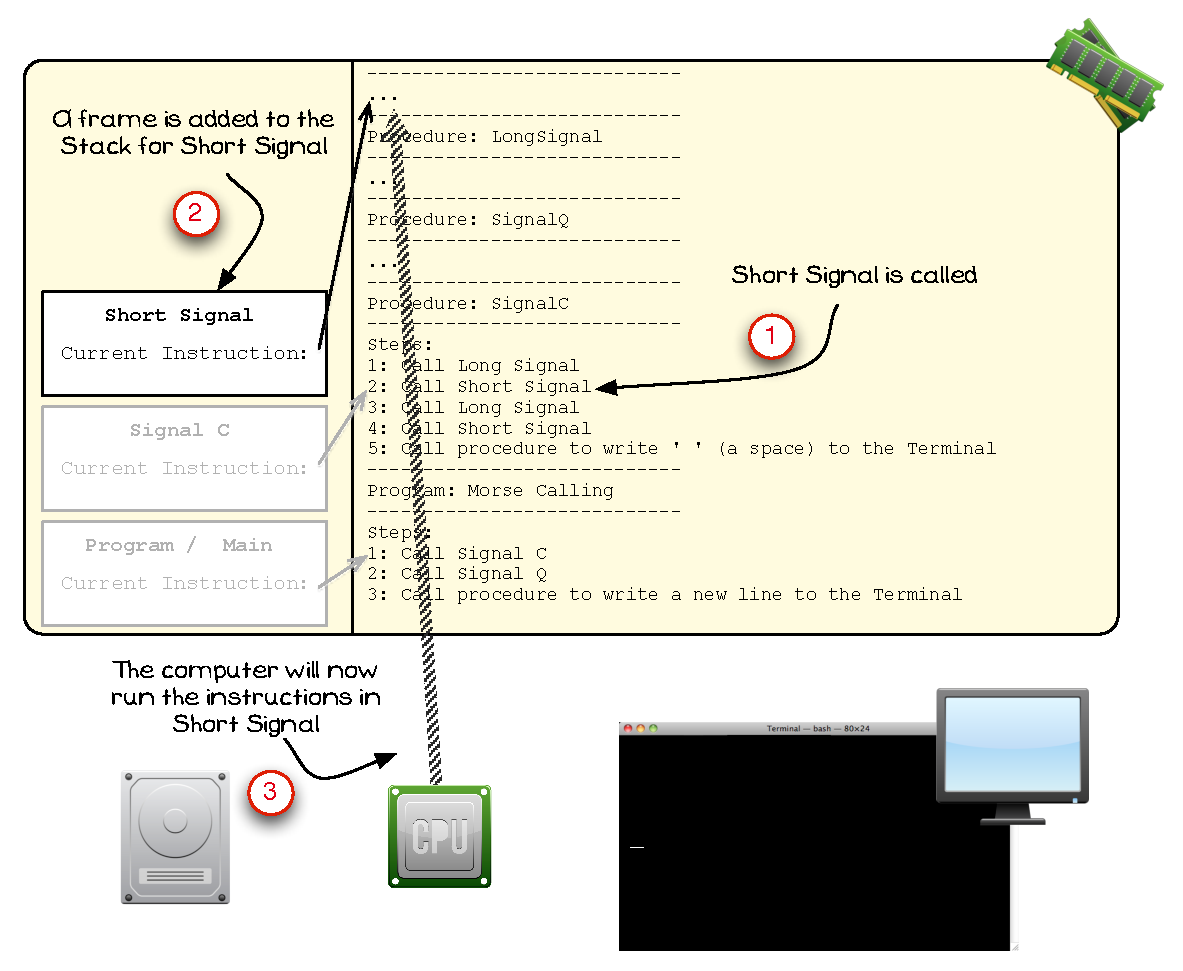
\includegraphics[width=\textwidth]{./topics/program-creation/images/ProcExe5} 
   \caption{\texttt{Short Signal} is called}
   \label{fig:procedure-decl-visualise-morsecalling-5}
\end{figure}

\mynote{
\begin{itemize}
  \item In Figure \ref{fig:procedure-decl-visualise-morsecalling-5} the indicated areas show the following:
  \begin{enumerate}
    \item The second instruction in the \texttt{Signal C} is a call to \texttt{Short Signal}.
    \item When this is executed a frame is added to the Stack to keep track of the current instruction within \texttt{Short Signal}'s code.
    \item As \texttt{Short Signal} is now on top of the Stack its instructions are executed.
  \end{enumerate}
  \bigskip
  
  \item In the \nameref{fig:procedure-decl-morsecalling-sequence} the program is now in the call to \texttt{Short Signal}.
\end{itemize}
}

% subsubsection short_signal_is_called (end)

\clearpage
\subsubsection{Short Signal Ends} % (fold)
\label{ssub:short_signal_ends}

When \texttt{Short Signal} ends control returns again to \texttt{Signal C}, with \texttt{Short Signal} having output a . to the Terminal.

\begin{figure}[htbp]
   \centering
   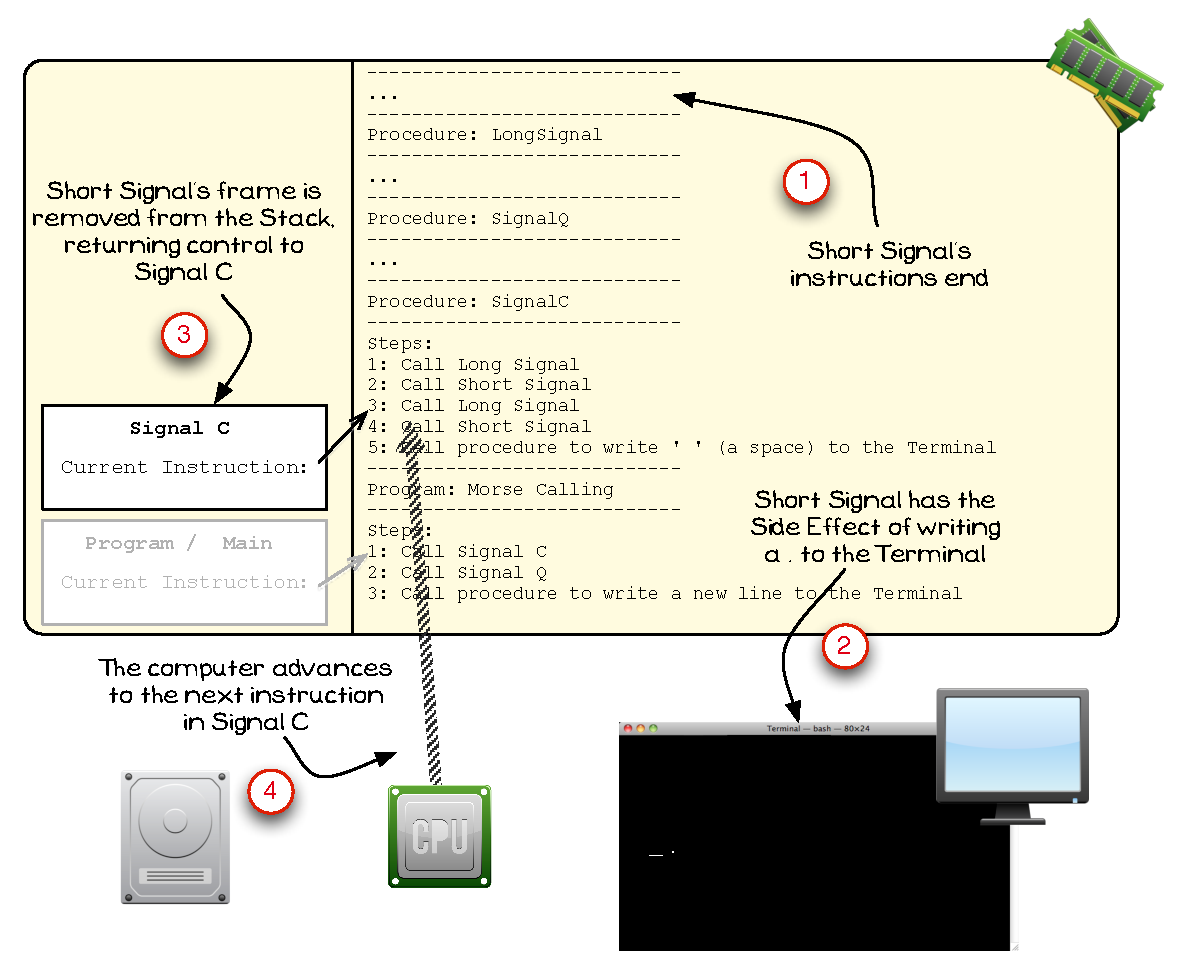
\includegraphics[width=\textwidth]{./topics/program-creation/images/ProcExe6} 
   \caption{\texttt{Short Signal} ends, returning control to \texttt{Signal C} again}
   \label{fig:procedure-decl-visualise-morsecalling-6}
\end{figure}

\mynote{
\begin{itemize}
  \item In Figure \ref{fig:procedure-decl-visualise-morsecalling-6} the indicated areas show the following:
  \begin{enumerate}
    \item The computer runs the instructions in \texttt{Short Signal} until they end.
    \item \texttt{Short Signal} has the \textbf{side effect} of writing an dot to the Terminal.
    \item When \texttt{Short Signal}'s instructions end control returns to \texttt{Signal C}.
    \item The computer now advanced to the next instruction in \texttt{Signal C}, the third Statement in the code.
  \end{enumerate}
\end{itemize}
}

% subsubsection short_signal_ends (end)

\clearpage
\subsubsection{Signal C runs to completion} % (fold)
\label{ssub:signal_c_runs_to_completion}

\texttt{Signal C} continues to run until it reaches the end of its instructions.

\begin{figure}[htbp]
   \centering
   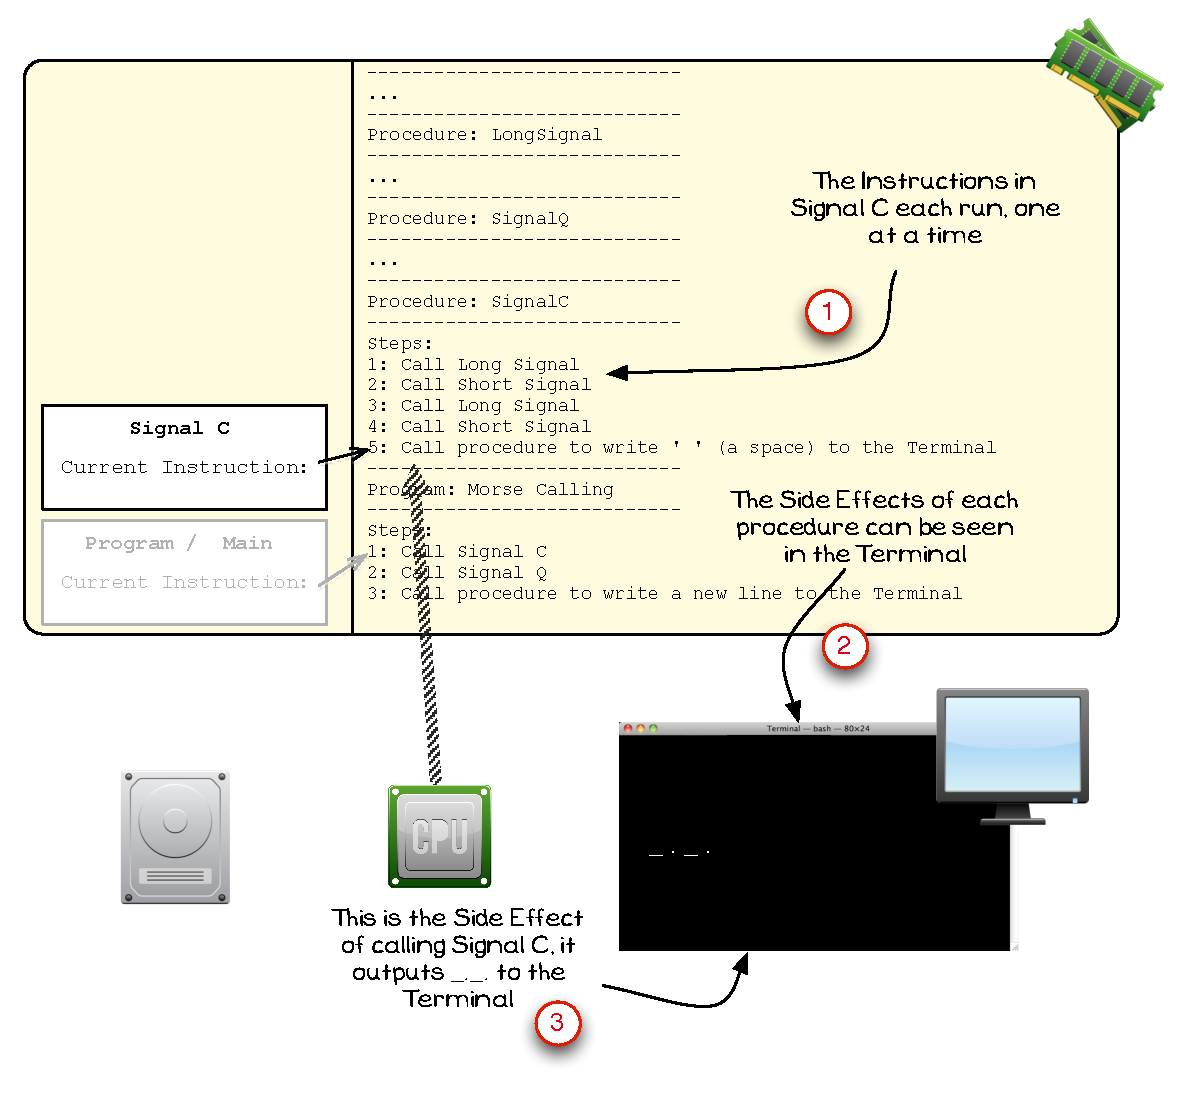
\includegraphics[width=\textwidth]{./topics/program-creation/images/ProcExe7} 
   \caption{\texttt{Signal C} runs until its instructions end}
   \label{fig:procedure-decl-visualise-morsecalling-7}
\end{figure}

\mynote{
\begin{itemize}
  \item In Figure \ref{fig:procedure-decl-visualise-morsecalling-7} the indicated areas show the following:
  \begin{enumerate}
    \item Each instruction in \texttt{Signal C} is run until all of the instructions in \texttt{Signal C} are complete.
    \item The side effects of the calls to \texttt{Long Signal} and \texttt{Short Signal} can be seen in the Terminal.
    \item The final state of the Terminal, showing {\morse C}, shows the side effect of calling \texttt{Signal C}.
  \end{enumerate}
\end{itemize}
}

% subsubsection signal_c_runs_to_completion (end)

\clearpage
\subsubsection{Signal Q is Called} % (fold)
\label{ssub:signal_q_is_called}

When \texttt{Signal C} finished the computer returns to the program's main instructions, where it moves on to the call to \texttt{Signal Q}.

\begin{figure}[htbp]
   \centering
   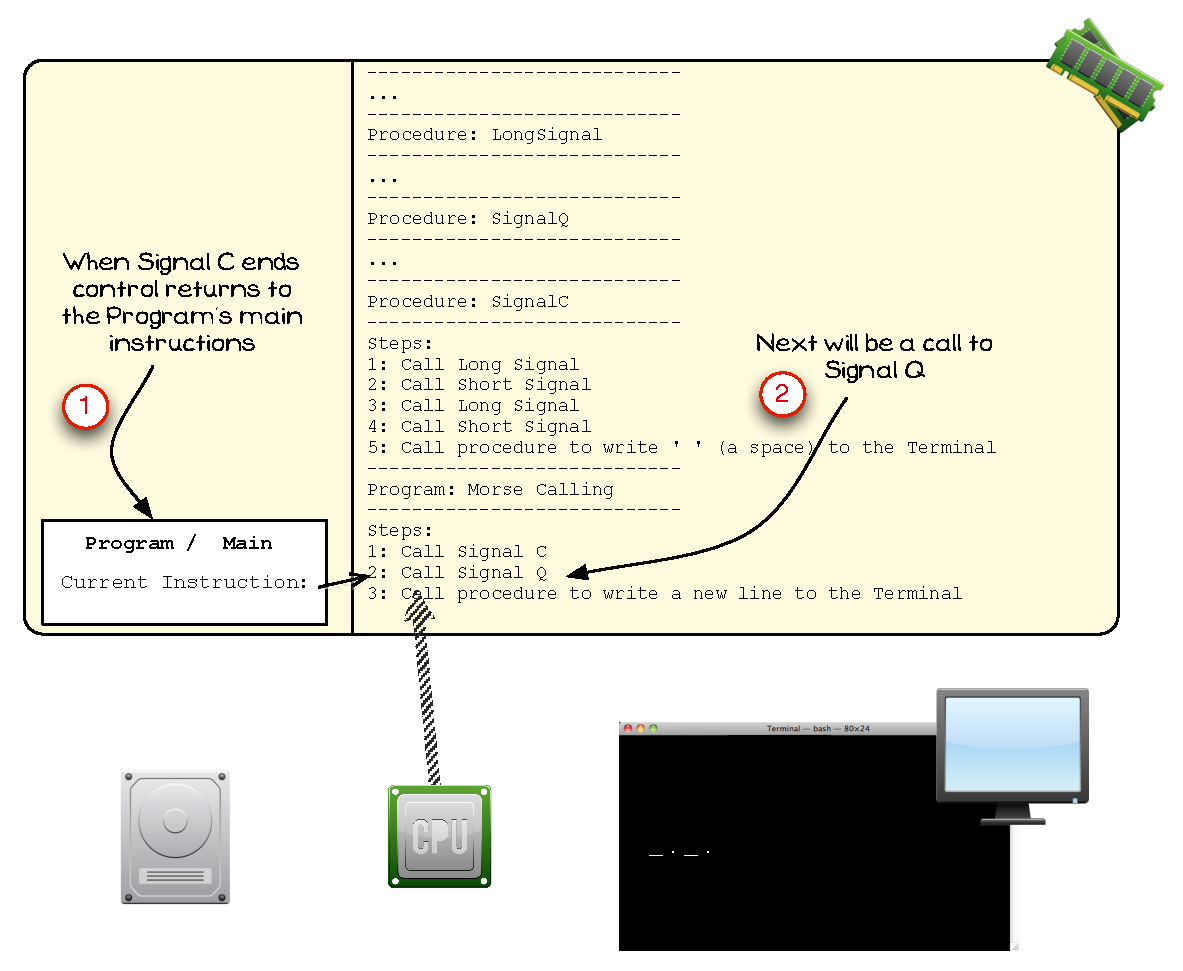
\includegraphics[width=\textwidth]{./topics/program-creation/images/ProcExe8} 
   \caption{}
   \label{fig:procedure-decl-visualise-morsecalling-8}
\end{figure}

\mynote{
\begin{itemize}
  \item In Figure \ref{fig:procedure-decl-visualise-morsecalling-8} the indicated areas show the following:
  \begin{enumerate}
    \item When \texttt{Signal C} ends its frame is removed from the Stack and control returns to the program's main instructions.
    \item The next call will be to \texttt{Signal Q}. The code in \texttt{Signal Q} will run, and output {\morse Q} to the Terminal, with each of the individual characters being written by the calls to \texttt{Long Signal} and \texttt{Short Signal} in the same way as it occurred in \texttt{Signal C}.
  \end{enumerate}
  
  \bigskip
  \item If you look at the \nameref{fig:procedure-decl-morsecalling-sequence} you can see that this is the point where control has returned to main, before it calls into \texttt{Signal Q}.
\end{itemize}
}

% subsubsection signal_q_is_called (end)
% subsection visualising_procedure_calls (end)

\clearpage
\subsection{Using this to Create Procedures} % (fold)
\label{sub:using_this_to_create_procedures}

Section \ref{sub:procedure_calls_in_action}, \nameref{sub:procedure_calls_in_action}, showed the actions the computer performs in order to execute the procedures that we create, but how does this information help us create our own programs and procedures?

One important aspect about procedures is the fact that they are \textbf{isolated} from each other. Notice that \texttt{Long Signal} does not care who called it, it is responsible for performing a \emph{long signal} and carries out this task when it is called. Similarly, \texttt{Short Signal} does not care who called it, it is responsible for performing a \emph{short signal} and carries out this task when it is called. Look back at the illustrations of execution and you should be able to see each Procedure carrying out its actions before control returns to where the procedure was called. In each case the called Procedure finishes the task it is responsible for performing before it ends.

This isolation also works in the other direction. \texttt{Signal C} calls \texttt{Long Signal} when it needs a \emph{long signal} to be performed. It does not care about how \texttt{Long Signal} achieves this, and can reply upon the fact that \texttt{Long Signal} will take care of its responsibilities before it ends. When you are working on designing or coding \texttt{Signal C} you focus on the task that \texttt{Signal C} needs to perform and make use of the other Procedures without needing to worry about how these Procedures achieve their responsibilities internally.

For Software Design and Development the isolated nature of procedures means that you can, and should, focus on the Procedure you are working on and ignore details of how other procedures work internally. 


\mynote{
\begin{itemize}
  \item A Procedure has \textbf{responsibilities}. It is responsible for performing some actions to create a certain side effect.
  \item Each Procedure is \textbf{isolated} from the other code in your program. 
  \item Focus on the Procedure you are designing or implementing, get it to meet its responsibilities and you will be one Procedure closer to your solution. Repeat this process for each Procedure in your design.
\end{itemize}
}

% subsection using_this_to_create_procedures (end)

\subsection{Summary} % (fold)
\label{sub:visualise-morse-calling-summary}

This Section has covered the use of \textbf{Structure Charts} and \textbf{Sequence Diagrams} to help visualise the relationships between procedures in a program, and to see how these Procedures work dynamically. This was supported by the illustration of how Procedures are executed by the computer.

\mynote{
The key messages to take away from this Section are:
\begin{itemize}
  \item A Procedure has the responsibility to perform a given task.
  \item The Procedure's name should reflect the task it performs.
  \item A \textbf{Structure Chart} shows the Procedures in a program, and how they are connected by procedure calls.
  \item The dynamic behaviour of the program can be shown using a \textbf{Sequence Diagram}, this sequence of procedure calls within the program.
  \item When a Procedure is called its instructions are followed. These instructions get the computer to perform the task the Procedure is responsible for.
  \item Procedures should cause \textbf{side effects}, changing something as a result of being called.
  \item Making sure each Procedure performs a \textbf{single task} will make your job easier.
  \item A \emph{single task} may have sub tasks that can be coded in their own procedures. For example, \texttt{Signal C} has sub tasks for performing long and short signals that can be coded into their own Procedures.
\end{itemize}
}

% subsection summary (end)

% section understanding_procedure_declaration_and_calls (end)

% ====================
% = Examples Section =
% ====================
\clearpage
\section{Procedure Declaration Examples} % (fold)
\label{sec:procedure_declaration_examples}

\subsection{Knock Knock} % (fold)
\label{sub:knock_knock}

This program prints out a short \emph{knock knock} joke to the Terminal. 
\begin{itemize}
  \item The description of the program is in Table \ref{tbl:procedure-decl-joke}
  \item The pseudocode is in Listing \ref{lst:procedure-decl-joke-pseudo}
  \item Figure \ref{fig:procedure-decl-tell-joke-struct} shows the Structure Chart for the Program
  \item The dynamic behaviour of the program is shown in the Sequence Diagram in Figure \ref{fig:procedure-decl-tell-joke-seq}
  \item Listing \ref{lst:procedure-decl-tell-joke-c} has the C code for the Program
  \item Listing \ref{lst:procedure-decl-tell-joke-pas} has the Pascal code for the Program
\end{itemize}

\begin{table}[h]
\centering
\begin{tabular}{l|p{10cm}}
  \hline
  \multicolumn{2}{c}{\textbf{Program Description}} \\
  \hline
  \textbf{Name} & \emph{Tell Joke} \\
  \\
  \textbf{Description} & Tells a joke using Procedures. \\
  \hline
\end{tabular}
\caption{Description of the Tell Joke program}
\label{tbl:procedure-decl-joke}
\end{table}

\begin{figure}[h]
   \centering
   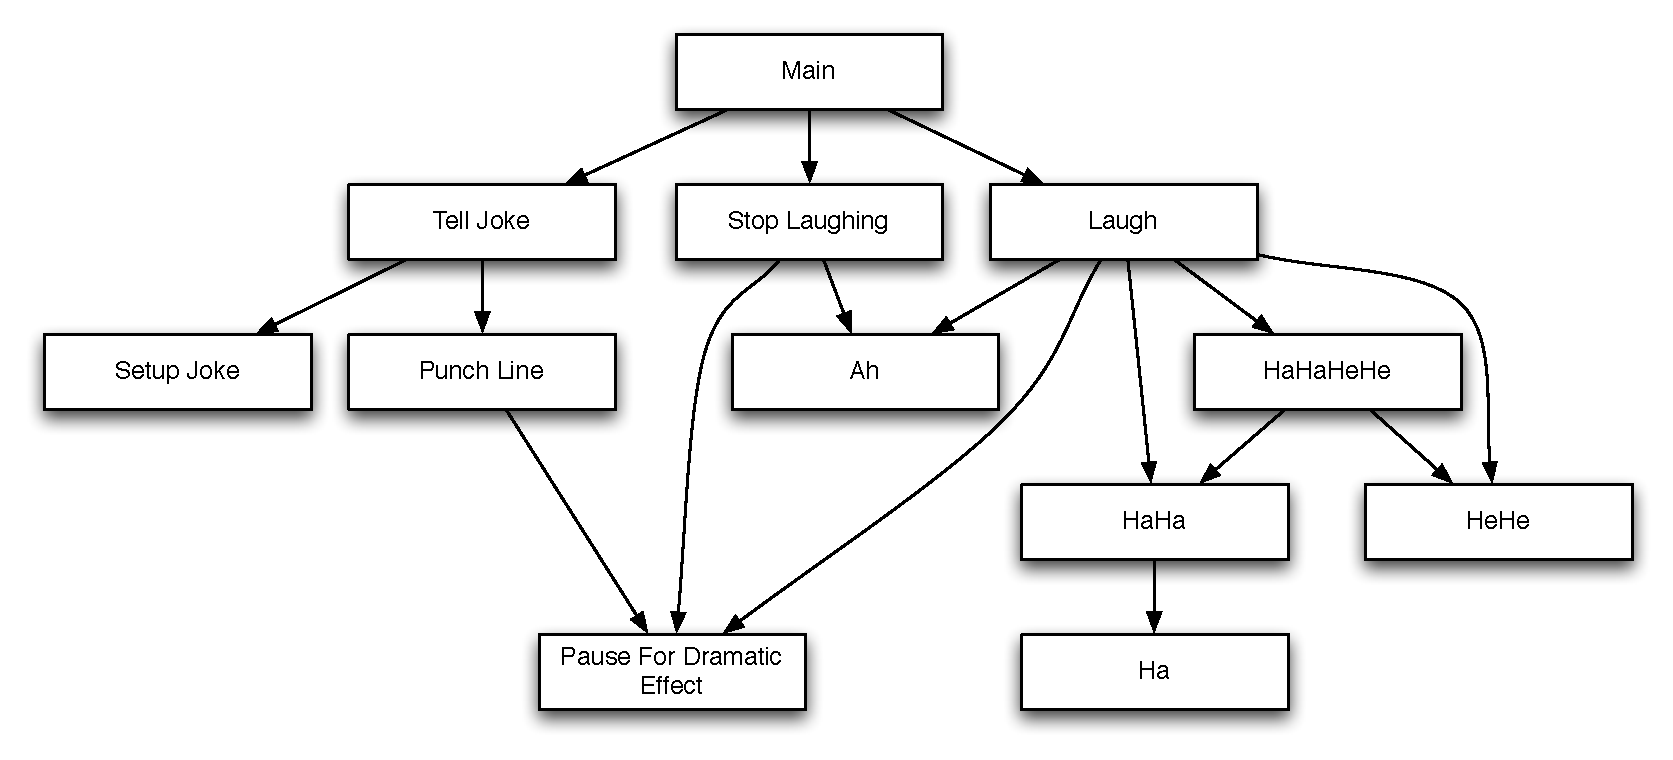
\includegraphics[width=\textwidth]{./topics/program-creation/images/TellJokeStructure} 
   \caption{Structure Chart for Tell Joke}
   \label{fig:procedure-decl-tell-joke-struct}
\end{figure}

\csection{The C language does not have a standard \emph{pause} or \emph{delay} procedure, instead of pausing execution the C version will just print ".. pause .." to the Terminal.}

\passection{In Pascal you can use the \texttt{CRT} unit to access a \texttt{Delay} procedure that pauses execution.}

\begin{figure}[p]
   \centering
   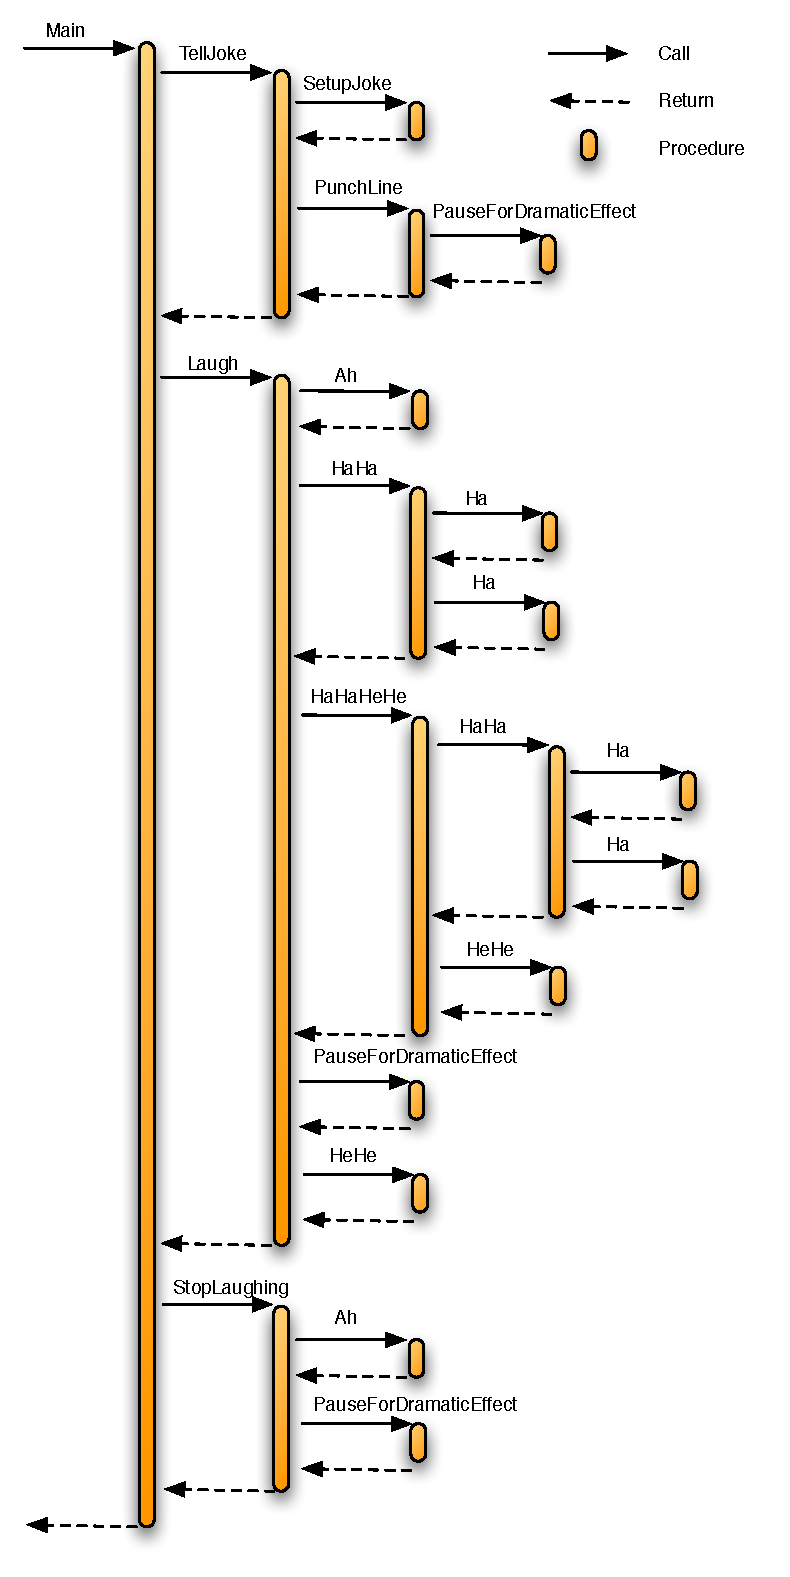
\includegraphics[width=0.7\textwidth]{./topics/program-creation/images/TellJokeSeq} 
   \caption{Sequence Diagram for Tell Joke}
   \label{fig:procedure-decl-tell-joke-seq}
\end{figure}


\lpseudocode{lst:procedure-decl-joke-pseudo}{Pseudocode for Tell Joke program.}{./topics/program-creation/examples/TellJoke.txt}{2}

\lcsection{\mccode{lst:procedure-decl-tell-joke-c}{C Knock Knock Joke}{topics/program-creation/examples/tell-joke.c}{2}}

\lpassection{\mpascode{lst:procedure-decl-tell-joke-pas}{Pascal Knock Knock Joke}{topics/program-creation/examples/TellJoke.pas}{2}}


% subsection knock_knock (end)

\subsection{Audio Morse Code} % (fold)
\label{sub:audio_morse_code}

This Chapter explained the development of a \emph{Morse Calling} program that output text to the Terminal. This version of the program uses \textbf{SwinGame} to play audio for the \emph{long} and \emph{short} signals.
\begin{itemize}
  \item The description of the program is in Table \ref{tbl:procedure-decl-morse-audio}
  \item The pseudocode is in Listing \ref{lst:procedure-decl-morse-audio-pseudo}
  \item The Structure Chart is very similar to the version that wrote its output to the Terminal, see Figure \ref{fig:procedure-decl-morsecalling-structure}. This code also include a \texttt{LoadSounds} procedure called from \texttt{Main}.
  \item The dynamic behaviour is the same as the the Sequence Diagram in Figure \ref{fig:procedure-decl-morsecalling-sequence}
  \item Listing \ref{lst:procedure-morse-calling-audio-c} has the C code for the Program
  \item Listing \ref{lst:procedure-morse-calling-audio-pas} has the Pascal code for the Program
\end{itemize}

\begin{table}[h]
\centering
\begin{tabular}{l|p{10cm}}
  \hline
  \multicolumn{2}{c}{\textbf{Program Description}} \\
  \hline
  \textbf{Name} & \emph{Morse Calling} \\
  \\
  \textbf{Description} & Plays audio for the morse code of `\emph{Calling Anyone}'. \\
  \hline
\end{tabular}
\caption{Description of the Morse Calling program}
\label{tbl:procedure-decl-morse-audio}
\end{table}

\csection{
\emph{SwinGame} has the following procedures that can help you implement this program:
\begin{itemize}
  \item \texttt{\textbf{play\_sound\_effect}}: you pass it the name of the sound effect to play.
  \item \texttt{\textbf{delay}}: allows you to pause execution for a number of milliseconds.
  \item \texttt{\textbf{load\_sound\_effect\_named}}: you pass it the name to use, and the filename to load. SwinGame will load the file from \emph{Resources/Sounds}.
  \item \texttt{\textbf{open\_audio}}: starts SwinGame's audio system, you cannot load or play sounds until after this is called.
  \item \texttt{\textbf{close\_audio}}: closes SwinGame's audio system, needed at the end of the program to match the \texttt{open\_audio}.
  \item \texttt{\textbf{release\_all\_resources}}: releases the loaded sound effects.
\end{itemize}
}

\passection{
\emph{SwinGame} has the following procedures that can help you implement this program:
\begin{itemize}
  \item \texttt{\textbf{PlaySoundEffect}}: you pass it the name of the sound effect to play.
  \item \texttt{\textbf{Delay}}: allows you to pause execution for a number of milliseconds.
  \item \texttt{\textbf{LoadSoundEffectNamed}}: you pass it the name to use, and the filename to load. SwinGame will load the file from \emph{Resources/Sounds}.
  \item \texttt{\textbf{OpenAudio}}: starts SwinGame's audio system, you cannot load or play sounds until after this is called.
  \item \texttt{\textbf{CloseAudio}}: closes SwinGame's audio system, needed at the end of the program to match the \texttt{OpenAudio}.
  \item \texttt{\textbf{ReleaseAllResources}}: releases the loaded sound effects.
\end{itemize}
}

\clearpage
\pseudocode{lst:procedure-decl-morse-audio-pseudo}{Pseudocode for Morse Calling with Audio.}{./topics/program-creation/examples/MorseCalling.txt}


\clearpage
\csection{\ccode{lst:procedure-morse-calling-audio-c}{C Audio Version of Morse Calling}{topics/program-creation/examples/morse-calling.c}}

\passection{\pascode{lst:procedure-morse-calling-audio-pas}{Pascal Audio Version of Morse Calling}{topics/program-creation/examples/MorseCalling.pas}}


% subsection audio_morse_code (end)
\clearpage
\subsection{Draw Sun Scene} % (fold)
\label{sub:draw_sun}

This small \textbf{SwinGame} creates a procedure to draw a sun in the top left corner of the screen.
\begin{itemize}
  \item The description of the program is in Table \ref{tbl:procedure-decl-draw-sun}
  \item The pseudocode is in Listing \ref{lst:procedure-decl-draw-sun-pseudo}
  \item Listing \ref{lst:procedure-draw-sun-c} has the C code for the Program
  \item Listing \ref{lst:procedure-draw-sun-pas} has the Pascal code for the Program
\end{itemize}

\begin{table}[h]
\centering
\begin{tabular}{l|p{10cm}}
  \hline
  \multicolumn{2}{c}{\textbf{Program Description}} \\
  \hline
  \textbf{Name} & \emph{Morse Calling} \\
  \\
  \textbf{Description} & Draws a simple scene where a sun is drawn in the upper left corner of the screen. \\
  \hline
\end{tabular}
\caption{Description of the Draw Sun Scene program}
\label{tbl:procedure-decl-draw-sun}
\end{table}

\csection{
\emph{SwinGame} has the following procedures that can help you implement this program:
\begin{itemize}
  \item \texttt{\textbf{open\_graphics\_window}}: you pass it the title of the window, and a width and height in pixels.
  \item \texttt{\textbf{delay}}: allows you to pause execution for a number of milliseconds.
  \item \texttt{\textbf{load\_sound\_effect\_named}}: you pass it the name to use, and the filename to load. SwinGame will load the file from \emph{Resources/Sounds}.
  \item \texttt{\textbf{clear\_screen\_to}}: clears the screen to the indicated color.
  \item \texttt{\textbf{refresh\_screen}}: displays the screen. All SwinGame drawing is performed in the background, this displays the screen to the user.
  \item \texttt{\textbf{draw\_circle}} and \texttt{\textbf{fill\_circle}}: draws the outline or fills a circle on the screen. This is passed the color of the circle, its x and y locations, and its radius.
  \item \texttt{\textbf{draw\_line}}: draws a line from one point to another. This is passed the color of the line, the x and y coordinates of the start point, and the x and y coordinates of the end point.
  \item \texttt{\textbf{release\_all\_resources}}: releases the loaded sound effects.
\end{itemize}
}

\passection{
\emph{SwinGame} has the following procedures that can help you implement this program:
\begin{itemize}
  \item \texttt{\textbf{OpenGraphicsWindow}}: you pass it the title of the window, and a width and height in pixels.
  \item \texttt{\textbf{Delay}}: allows you to pause execution for a number of milliseconds.
  \item \texttt{\textbf{ClearScreen}}: clears the screen to the indicated color.
  \item \texttt{\textbf{RefreshScreen}}: displays the screen. All SwinGame drawing is performed in the background, this displays the screen to the user.
  \item \texttt{\textbf{DrawCircle}} and \texttt{\textbf{FillCircle}}: draws the outline or fills a circle on the screen. This is passed the color of the circle, its x and y locations, and its radius.
  \item \texttt{\textbf{DrawLine}}: draws a line from one point to another. This is passed the color of the line, the x and y coordinates of the start point, and the x and y coordinates of the end point.
  \item \texttt{\textbf{ReleaseAllResources}}: releases the loaded sound effects.
\end{itemize}
}

\mynote{
SwinGame colors are \texttt{ColorBlue, ColorGreen, ColorRed, ColorWhite, ColorBlack, ColorYellow,
ColorPink, ColorTurquoise, ColorGrey, ColorMagenta, and ColorLightGrey}.
}


\clearpage
\pseudocode{lst:procedure-decl-draw-sun-pseudo}{Pseudocode for Draw Sun Scene program}{./topics/program-creation/examples/draw-sun.txt}


\clearpage
\csection{\ccode{lst:procedure-draw-sun-c}{C Draw Sun Scene Program}{topics/program-creation/examples/draw-sun.c}}

\passection{\pascode{lst:procedure-draw-sun-pas}{Pascal Draw Sun Scene Program}{topics/program-creation/examples/DrawSun.pas}}



% subsection draw_sun (end)


% section procedure_declaration_examples (end)

% =============
% = Exercises =
% =============
\clearpage
\section{Procedure Declaration Exercises} % (fold)
\label{sec:procedure_declaration_exercises}

\subsection{Concept Questions} % (fold)
\label{sub:concept_questions_proc}

Read over the concepts in this chapter and answer the following questions:
\begin{enumerate}
  \item What is a \nameref{sub:program}? What does it contain?
  \item What is a \nameref{sub:procedure}? What does it contain?
  \item If \texttt{Main} calls \texttt{Draw Scene}, and \texttt{Draw Scene} calls \texttt{Draw Sun}, what order must these procedures be declared in your program's code?
  \item Why create your own procedure? Why not just code all the instructions in the one main procedure?
  \item It is stated that a procedure should have a side effect, what does this mean?
  \item Examine the `Tell Joke' program, see \sref{sub:knock_knock}, then answer the following questions.
  \begin{enumerate}
    \item How many times is the \texttt{Ha} procedure called?
    \item How many times is the \texttt{Ha} procedure written? What does this mean for the use of procedures in our code?
    \item At its deepest, how many stack frames will be on the stack when the `Tell Joke' program is run?
    \item Which procedures call \texttt{Pause For Dramatic Effect}?
    \item What does the name of each procedure tell us?
  \end{enumerate}
  \item Picture yourself in the following scenario, and then answer the following questions.
  \begin{quote}
    As a graduate you start work as a software developer in a startup building some really cool software. The project that you are working on has around 100 features, which are implemented in 10,000 procedures. You are asked to fix a specific bug in the program. 
    \begin{itemize}
      \item This bug effects just a single feature. 
      \item The other developers believe that the issue is located in a single procedure but they want you to learn how the program is structured, so they will not tell you which procedure it is. 
      \item You have played with the software and you know how to cause the bug.
      \item There are about four or five steps from the program's start, up to the point where the bug occurs.    
    \end{itemize}
  \end{quote}
  \begin{enumerate}
    \item When you get the code, what strategy would you use to locate the one procedure that has the bug?
    \item Would you need to understand all ten thousand procedure? Explain your reasoning.
    \item Do you think you would need to read the procedures called by the procedure with the bug? Explain your reasoning.
    \item When you understand the section of the code related to the bug you will need to implementing a fix. Explain why you would be able to focus your attention to this one procedure when you are implementing the fix.
    \item How would you test that your fix has solved the problem?
    \item The next bug you need to fix occurs across a number of different features of the program. The cause is still expected to exist within a single procedure. How would this change the way that you approach locating and fixing the bug?
  \end{enumerate}
  
\end{enumerate}
% subsection concept_questions (end)

\clearpage
\subsection{Code Writing Questions: Applying what you have learnt} % (fold)
\label{sub:code_writing_questions_applying_what_you_have_learnt_proc}

Apply what you have learnt to the following tasks:
\begin{enumerate}
  \item Create a Morse SOS program that outputs the morse code for the distress signal to the Terminal. See \tref{tbl:procedure-decl-morse_sos}.
  
  \begin{table}[h]
  \centering
  \begin{tabular}{l|p{10cm}}
    \hline
    \multicolumn{2}{c}{\textbf{Program Description}} \\
    \hline
    \textbf{Name} & \emph{Morse SOS} \\
    \\
    \textbf{Description} & Displays the morse code for a distress signal on the Terminal. \\
    \hline
  \end{tabular}
  \caption{Description of the Morse SOS program.}
  \label{tbl:procedure-decl-morse_sos}
  \end{table}
  
  \item Create a Morse Name program that outputs your name in morse code to the Terminal. See \tref{tbl:procedure-decl-morse_name}.
  
  \begin{table}[h]
  \centering
  \begin{tabular}{l|p{10cm}}
    \hline
    \multicolumn{2}{c}{\textbf{Program Description}} \\
    \hline
    \textbf{Name} & \emph{Morse Name} \\
    \\
    \textbf{Description} & Displays the morse code for your name on the Terminal. \\
    \hline
  \end{tabular}
  \caption{Description of the Morse Name program.}
  \label{tbl:procedure-decl-morse_name}
  \end{table}
  
  \item Update your Morse SOS program to use SwinGame, and either flash the screen to signal your message or play morse code sound effects.
  \item Update your Morse Name program to use SwinGame, and either flash the screen to signal your message or play morse code sound effects.
  
  \item Take the Seventy Three Times Table program from \cref{cha:program_creation}, and re-implement it so that it has a \texttt{Print Times Table} procedure.
  \item Take the Face Shape program from \cref{cha:program_creation}, and re-implement it so that the face is drawn in a \texttt{Draw Face} procedure.
  \item Download the code for the Scene Drawing program from the website, and rewrite it to make use of Procedures.
\end{enumerate}
% subsection code_writing_questions_applying_what_you_have_learnt (end)

\bigskip
\subsection{Extension Questions} % (fold)
\label{sub:extension_questions_proc}

If you want to further your knowledge in this area you can try to answer the following questions. The answers to these questions will require you to think harder, and possibly look at other sources of information.
\begin{enumerate}
  \item Are the procedures in the libraries any different from the procedures you create?
  \item Explore the procedures that are available to you in the standard library that comes with your language. Name some of the procedures you think will be useful to know about in the future.
  \item Explore the procedures that are available to you in the SwinGame library. Name some of the procedures you think will be useful to know about in the future.
  \item Why must procedures have side effects?
  \item How should procedures be named?
\end{enumerate}

% subsection extension_questions (end)

% section procedure_declaration_exercises (end)

% ===================
% = Project Section =
% ===================
% \clearpage
% \section{Procedure Declaration Project} % (fold)
% \label{sec:procedure_declaration_project}



% section procedure_declaration_project (end)
% chapter procedure_declaration (end)